\documentclass[10pt]{report}
\usepackage{fullpage}
\usepackage{times}
\usepackage{amsmath,proof,amsthm,amssymb,color}
%\usepackage{multicol}
\usepackage{float}
\usepackage{graphicx}
\usepackage{parskip}
\floatstyle{boxed} 
\restylefloat{figure}
\usepackage{hyperref}
\usepackage{listings}
%\usepackage[all]{hypcap}

\setcounter{secnumdepth}{3}
\setcounter{tocdepth}{1}


\title{{\Huge virtexsquared:}\\an ARM-like System-on-Chip on an FPGA}

\author{Joshua Wise\\
\texttt{$<$jwise@andrew.cmu.edu$>$} \and
Josiah Boning\\
\texttt{$<$jboning@andrew.cmu.edu$>$} \and
Bradley Yoo\\
\texttt{$<$bjy@andrew.cmu.edu$>$}}


\begin{document}
\maketitle

\begin{abstract}

The authors provide a report on the completed development of an ARM-like
System-on-Chip built on a Xilinx Virtex-5 FPGA.  A high-level overview of
the design is provided, as well as detailed examinations of various
submodules within the system.  An examination of both the hardware and
software stack is provided, and the authors take a moment to reflect.

\end{abstract}

\tableofcontents

\chapter{Introduction}

In fulfillment of the 18-545 Advanced Digital Design Capstone, this group
designed and implemented a System on a Chip on an FPGA, based around a small
ARM-like core.  The system is built around two memory buses, and contains
I/O cores to interface with a smattering of peripherals, including:

\begin{itemize}
\item{DVI/VGA output from Chrontel CH7301C, for which video is cached in a
framebuffer in main memory;}
\item{RS-232 serial output;}
\item{AC'97 audio with Analog AD1981B, for which audio to be output is cached in a
a simple main memory buffer;}
\item{PS/2 keyboard input;}
\item{CompactFlash via the Xilinx SystemACE controller;}
\item{and main memory via a DDR2 SODIMM, for which interface glue is
provided using Xilinx's predesigned Memory Interface Generator (MIG) IP.}
\end{itemize}

The system contains various non-I/O cores to provide additional functionality,
including:

\begin{itemize}
\item{a cycle counter for precise application timing;}
\item{a preloader to load the initial bootstrap into RAM;}
\item{and memory set and image blit accelerators.}
\end{itemize}

A primary goal of this peripheral layer is to be reused in 18-447; the system
is designed to be simple to interface with from a core perspective, and
hence usable for students in an introductory computer architecture class. 
The core, in particular, has a moderate \textit{anti}-goal of high
performance.

The system has been implemented over the course of the Fall 2010 semester to
the point of successfully executing a small rhythm game that shows off the
system's ability to render video in real time and the capability to
synchronize keyboard input with video and audio output; this completes the
original goal.

\chapter{Hardware Design}

\label{par:hardware}

In this part, we provide an overview of the design and implementation
decisions involved in the \textit{hardware} part of the system.  As a whole,
this section corresponds to the \texttt{rtl/} directory in the top level
source repository; the astute reader may follow along within.

\section{Memory Architecture}

\label{sec:memory}

The system, as a whole, is partitioned into two major access paths -- the
FSAB (\textit{Fast System Access Bus}), and the SPAM Bus (\textit{Slow
Peripheral Access Memory} Bus).  These two buses were designed to meet
wildly differing goals; the FSAB is designed for high-bandwidth, cachable
transactions, whereas the SPAMBus is designed for configuration space
register (CSR) accesses.  Ideally, most of the system's traffic will occur
over the FSAB.

\begin{figure}
  \centering
    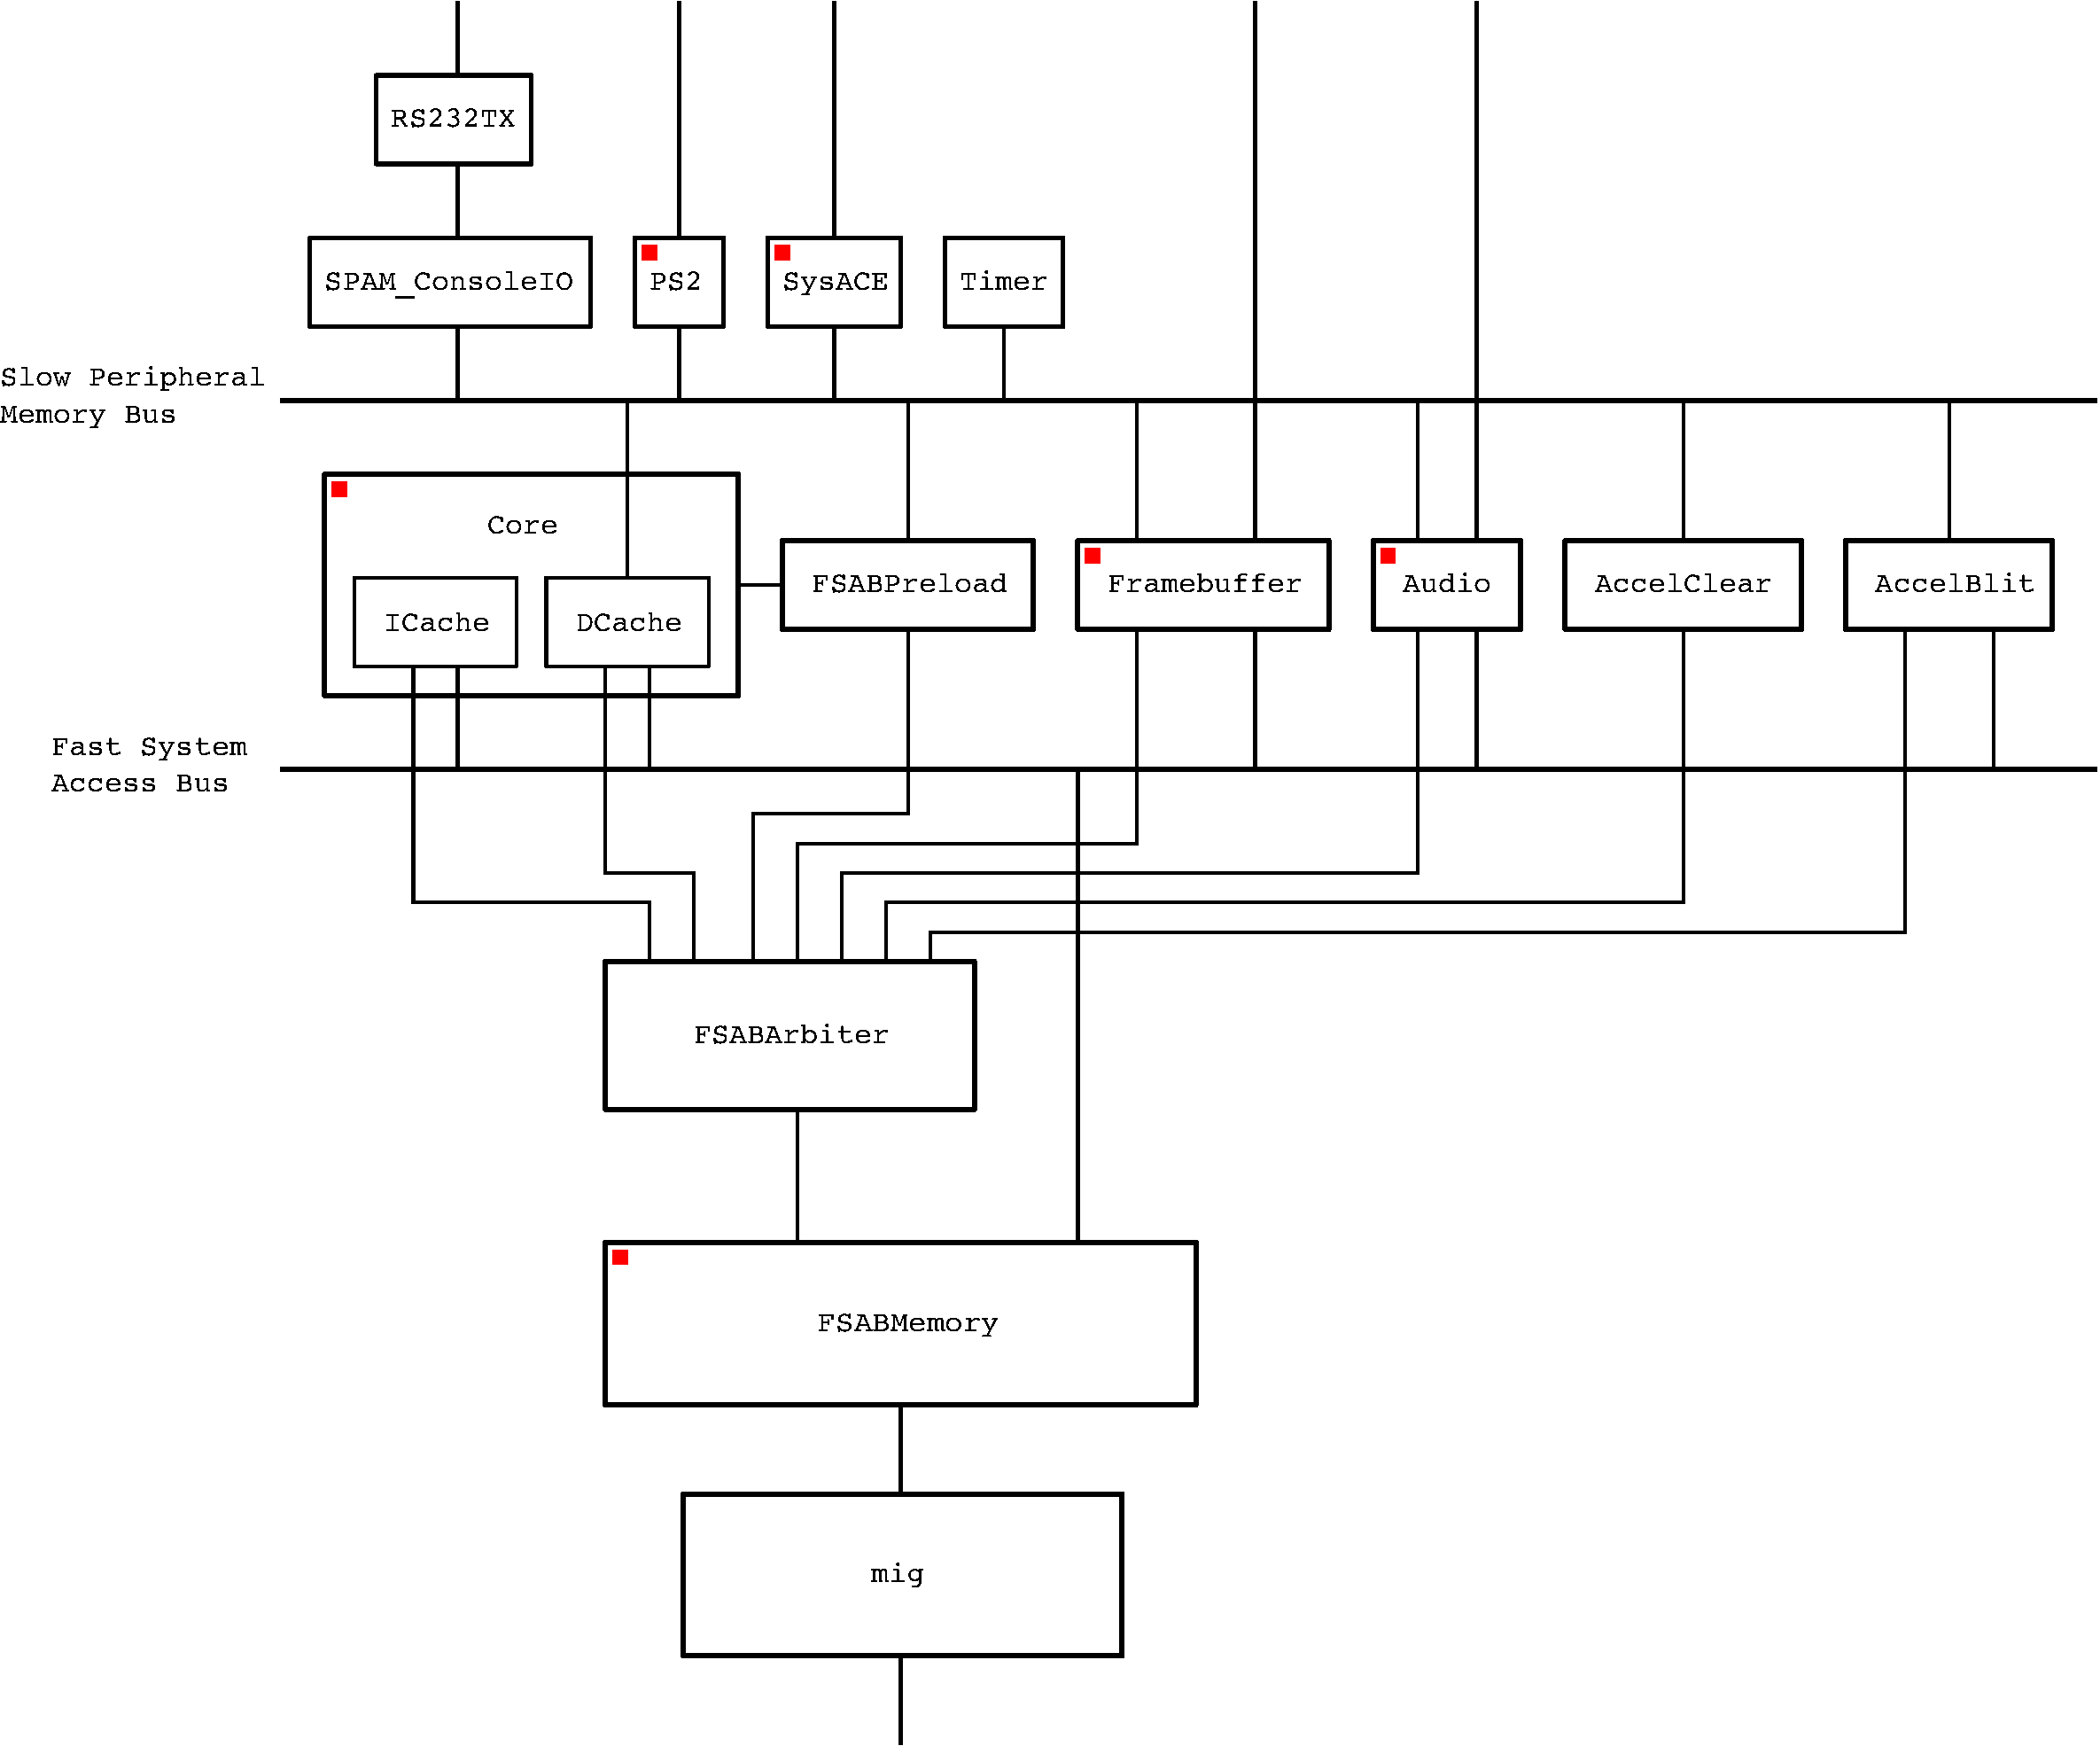
\includegraphics[width=.8\textwidth]{block_diagram.pdf}
  \caption{High-level system diagram. A red square in the corner of a module
           indicates a module where a ChipScope ILA is present and can easily
           be enabled.}
  \label{system_diagram}
\end{figure}

\subsection{Fast System Access Bus}

\label{sec:fsab}

The FSAB is a transaction-oriented bus designed primarily for accessing high-
latency memories such as DRAMs. The vast majority of the memory accesses on 
the system during normal operation (i.e., not at boot/ configuration time) 
will happen via the FSAB. 

\subsubsection{Terminology}

The FSAB works in terms of `transactions'. A read transaction shall consist 
of the `read request', and `read data' phases. A write transaction shall 
consist only of the `write data' phase.

Devices attached to the FSAB are classified as `masters' and `slaves'; a 
device that initiates transactions (reads and writes to main memory) is a 
master, and a device that completes transactions is a slave.

At times, it may be useful to discuss directions on the FSAB. For the purposes
of this discussion, data that is traveling from a master to a slave is 
considered `outbound' (and so signals for that purpose will begin with fsabo); 
similarly, data that initiates at the slave and returns to a master is 
considered `inbound' (and so signals for that purpose will begin with fsabi).


\subsubsection{Conceptual Overview}

virtexsquared, in its first incarnation, will only have a single memory 
controller. For that reason, the FSAB will be defined to have only one slave 
device - but since many peripherals may wish to do DMA access to or from main 
memory, the FSAB will be defined to potentially have many masters. The fact 
that only one slave device exists shall not be extensively exploited in either 
the design or implementation of the FSAB, since at a later time, a second 
memory controller may be interesting.

Since many memory controllers are capable of handling multiple pipelined 
requests, the FSAB supports multiple transactions in flight at a time. The 
slave will arbitrate these requests with a debit-credit system. Similarly, 
contention between masters will be resolved with an arbiter module that also 
performs queueing and debit-credit arbitration. In this regard, the bus 
arbiter should be ``invisible'' to a master; the debit-credit system should be 
interface-identical as if the master were talking directly to the slave.

Most operations that peripherals on the FSAB will perform will be in similar 
sizes. For instance, the I\$ and D\$ will always read sizes of a single cache 
line; the TLB will generally read page directory entries at a time; and the 
framebuffer will generally load half a FIFO's worth or so at a time. The 
general case, anyway, will not be a read of a single word. Similarly, writes 
will often be localized to each other. To facilitate this, each FSAB 
transaction will have a count of words up to a defined maximum of 8 along with 
the command and address. Inside each transaction, the address being written to 
shall autoincrement with each datum sent. Since not every datum may be 
interesting for a write, a ``write mask'' is also sent with every word written.

Since masters are isolated from each other by one or more arbiters, it is
generally not possible for one master to know what another master is doing.
Lacking any other form of cache coherency protocols (such as MOESI), a
system based around the FSAB is not cache-coherent! This means that the
applications programmer must take extra care to make sure that all data is
synchronized to main memory before allowing another peripheral to access
said data. (For instance, if the programmer wishes to write new data to the
frame buffer before flipping pages, he must cause the CPU to clean that
cache line by some mechanism first. In the current implementation, the data
cache is implemented as being write-through, so no such synchronization
issue takes place.)

The bus protocol is designed to be easy to implement by a DRAM-based slave. 
For that reason, the length of a read or write request is limited not just by 
the maximum, but by the alignment of the request. That is to say, if a request 
is only aligned to a four-qword boundary, but not to an eight-qword boundary, 
then the maximum size of the request is four qwords; a request of five or more 
qwords results in undefined behavior. (On the current DRAM-backed 
implementation, the resulting data comes from wrapping around the row buffer; 
on the current simulation-backed implementation, the resulting data comes from 
subsequent linear addresses.) 

\subsubsection{Design Overview: Portlist}

A FSAB master has the following ports outbound:

\begin{lstlisting}[basicstyle=\footnotesize,language=Verilog]
output                  fsabo_valid;
output [FSAB_REQ_HI:0]  fsabo_mode;
output [FSAB_DID_HI:0]  fsabo_did;
output [FSAB_DID_HI:0]  fsabo_subdid;
output [FSAB_ADDR_HI:0] fsabo_addr;
output [FSAB_LEN_HI:0]  fsabo_len;
output [FSAB_DATA_HI:0] fsabo_data;
output [FSAB_MASK_HI:0] fsabo_mask;
input                   fsabo_credit;
\end{lstlisting}

A FSAB master has the following ports inbound:

\begin{lstlisting}[basicstyle=\footnotesize,language=Verilog]
input                   fsabi_valid;
input  [FSAB_DID_HI:0]  fsabi_did;
input  [FSAB_DID_HI:0]  fsabi_subdid;
input  [FSAB_DATA_HI:0] fsabi_data;
\end{lstlisting}

No debit output (or input) is needed; a debit occurs implicitly when a new
FSAB transaction is begun. The credit input is always considered valid, even
if the inbound valid flag is not set.

\subsubsection{Design Overview: Transaction Specifics}

Transactions are defined by a start packet (and potentially additional data
packets) being sent to a slave, and the slave responding with any necessary
data packets. The slave may pipeline transactions as much as it is able
(credits can be returned before the slave has responded), but the slave
shall never reorder transactions. (Doing so would result in indeterminate
behavior with reads after writes, among other things.)

A start packet shall consist of the valid bit being set, the mode flag being
set to either FSAB\_READ or FSAB\_WRITE, the did/subdid set to the appropriate
values, an address, a length, and the first word of data and mask, should
they be valid for the current operation. Once a transaction is being sent
outbound, it shall not be interrupted by another transaction; the next data
packets are always part of this transaction. (For this reason, a master
should attempt to send packets as quickly as possible; excessive delay
between subsequent assertion of the valid flag may result in poor bus
performance.) In subsequent data packets, all control flags (i.e., all but
valid, data, and mask) are ignored.

The debit/credit system shall count each transaction as a debit, not each
word. Another transaction may be sent immediately after the credit flag is
asserted (or the credit may be queued).

The did field of each transaction shall be set as per each master's DID
assignment. The subdid may be set according to any internal state that the
master needs to track.

Some attention should be given to the mechanisms of clock distribution. In 
particular, it is permissible (and indeed often the case) that the inbound FSAB 
and outbound FSAB buses may be on different clock domains; usually the inbound 
FSAB clock comes directly from the slave, but the outbound FSAB clock is 
synchronous with the logic from the driving module. The outbound FSAB interface 
is then synchronized to the slave's clock in the arbiter. \footnote{This may be
considered a bug, as it departs from the conceptual goal that the bus arbiter 
is invisible to the master. From this perspective, it is preferable to have all
portions of the FSAB on the same clock domain, i.e. the slave's.}

\subsubsection{Known implementations}

The following are known implementations of the FSAB specification:

\begin{figure}
  \centering
    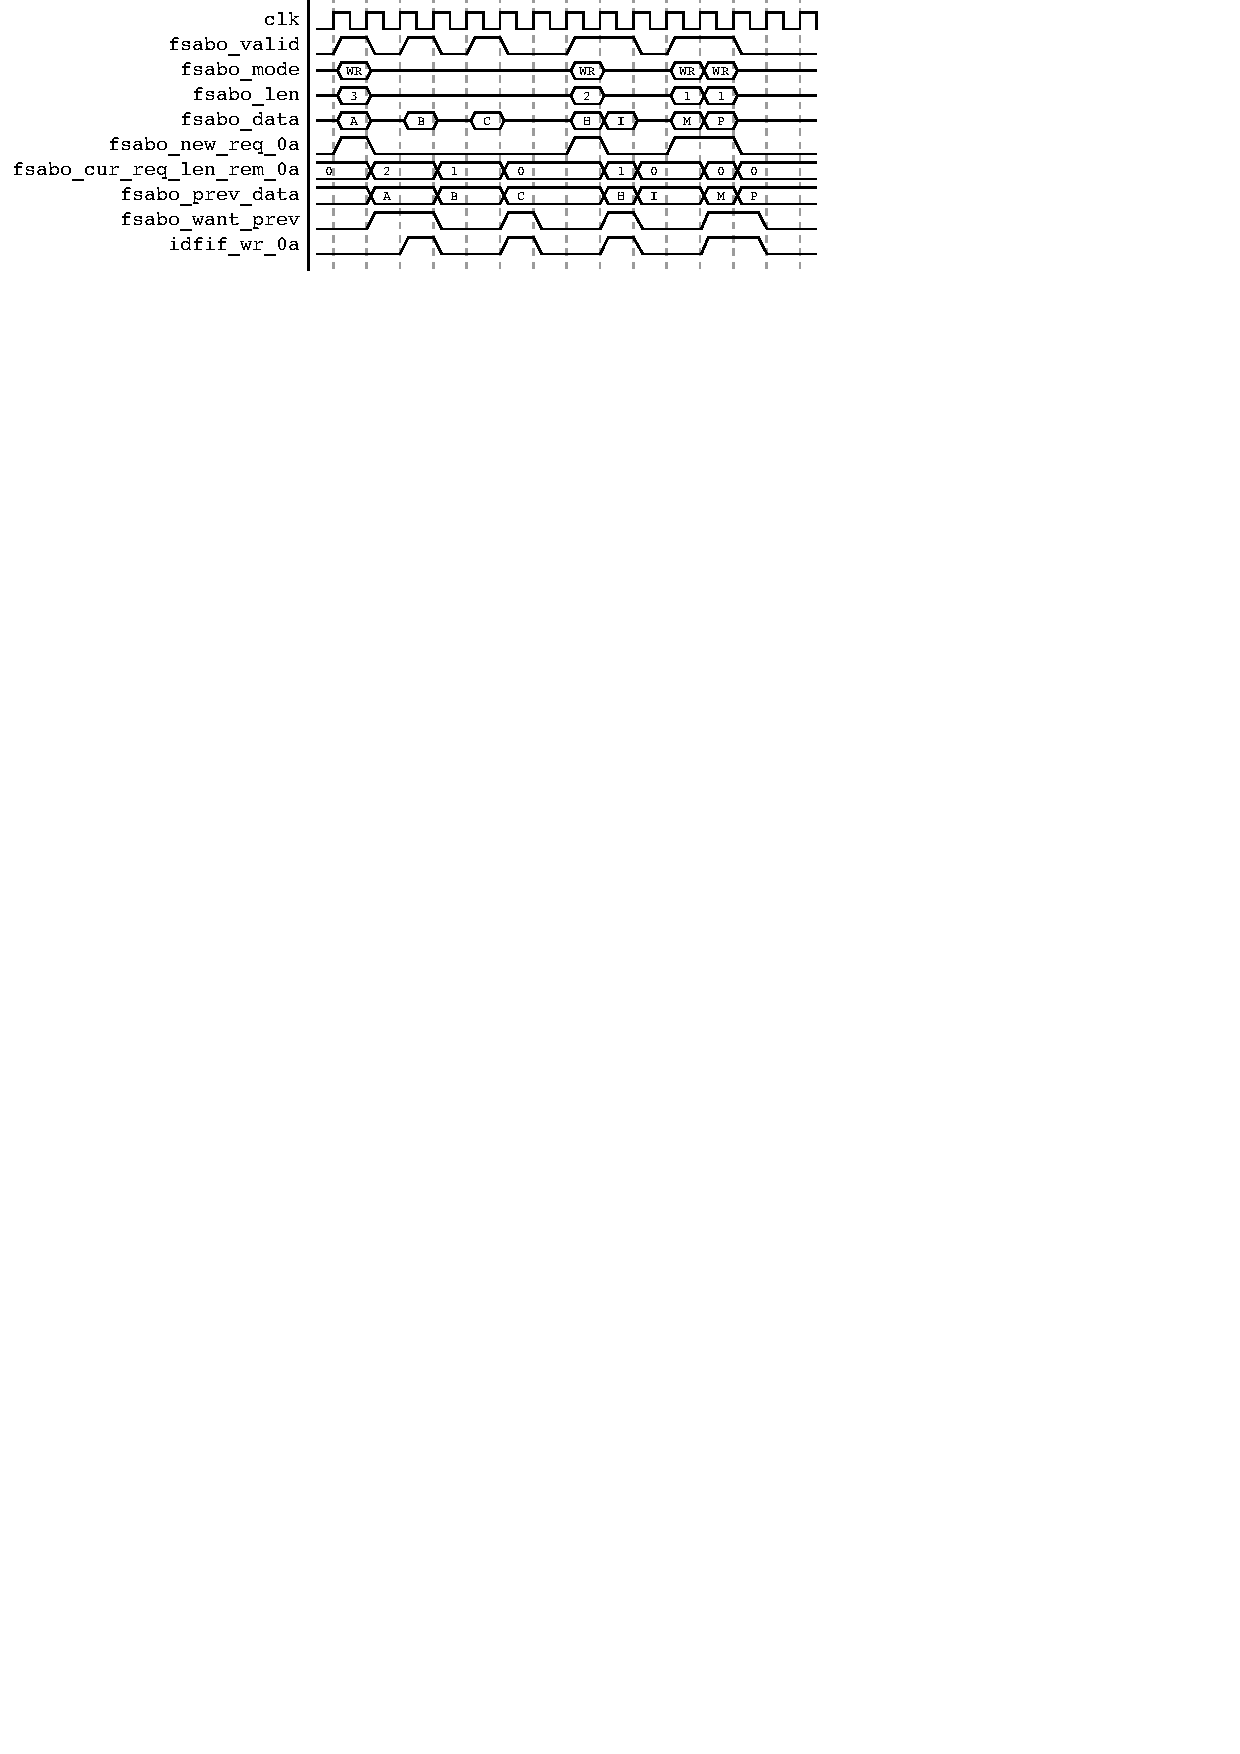
\includegraphics[width=0.85\textwidth]{FSAB-IxFIF.pdf}
  \caption{Clocking for memory controller.} \label{fsabixfif}
\end{figure}


\begin{itemize}
\item{Caches}
\item{Memory Controller}
\item{Arbiter}
\item{DMA Controller}
\end{itemize}

\subsection{Slow Peripheral Access Memory}
\label{sec:spam}

The SPAM bus is a word-oriented one-access-at-a-time bus designed primarily
for accessing configuration space registers (CSRs) on peripherals.

\subsubsection{Conceptual Overview}

In theory, all peripherals on the system will be matching and decoding on
the SPAM bus; when the processor does a SPAM-bus access, it is almost
certainly the case that a device will respond.  So, the bus should be
optimized for the common case in which a device responds shortly after a
request is sent.  Similarly, it should be the case that only one device ever
matches, so the bus need not be arbitrated between them; a simple OR'ing of
responses should work.

No peripheral should need to access any other peripheral's CSRs; any such
accesses from a debug interface should be multiplexed in between the CPU and
the SPAM-bus.  As such, the master-slave relationship in the SPAM-bus is
exactly the opposite of what it is on the FSAB; there is only one SPAM-bus
master, and there can be many SPAM-bus slaves.  Again, this property should
not be extensively exploited, but it is the case in the current
implementation.

Requests on the SPAM-bus should ordinarily be low latency, but there may be
need for wait states for various reasons.  For instance, if the other
peripheral is far away on the die, it may take an extra clock to compute the
appropriate response for a read.  A write, perhaps, may block until some
(short) action is complete.  There may also be a need to block because the
target peripheral is in a different clock domain, and a synchronizer needs
to shift the data over.

If no peripheral answers by deasserting busy\_b within a reasonable number
of cycles (usually 256), the request is deemed to have timed out, and a read
should return a value indicating that (usually something along the lines of
0xDEADDEAD).

\subsubsection{Design Overview: Portlist}

The processor has the following ports outbound:

\begin{lstlisting}[basicstyle=\footnotesize,language=Verilog]
output                  spamo_valid;
output                  spamo_r_nw;
output [SPAM_DID_HI:0]  spamo_did;
output [SPAM_ADDR_HI:0] spamo_addr;
output [SPAM_DATA_HI:0] spamo_data;
\end{lstlisting}

The processor has the following ports inbound:

\begin{lstlisting}[basicstyle=\footnotesize,language=Verilog]
input                   cio__spami_busy_b;
input  [SPAM_DATA_HI:0] cio__spami_data;
\end{lstlisting}

\subsubsection{Design Overview: Lifecycle of a request}

A request begins by the processor asserting the valid flag and specifying
the rest of the fields. This happens for exactly one cycle. Some time later
(potentially even on the same cycle), a device may assert the busy\_b flag
for one cycle to indicate that the request has been filled. Inbound data
shall be valid on the same cycle.

No new request shall be specified until either a previous request has returned, 
or a previous request has timed out. A request shall time out after no fewer 
than 128 cycles; the current DCache implementation times out after 256 cycles. 
When a device is not specifying data inbound, it shall drive its output port to 
zero; this allows the bus to simply OR together all responses.

Since the SPAM bus is always on the core's clock domain, some synchronization 
may be needed for CSRs on a different clock domain. Standard modules have been 
provided to synchronize reads and writes; for more information on those, see 
the documentation for the CSRAsync modules in section \ref{sec:csrasync}. 

\section{Core Microarchitecture}

As part of the virtexsquared system, the core must conform to the defined
bus protocols on the external interface (see section \ref{sec:memory}); but
within the core itself, anything goes.  Although the ARM core will not be
reused in future projects, the caches and global interface will be, and
hence potentially merit discussion.

\subsection{ARM Core}

The ARM core consists of the register file, fetch, decode, issue, execute,
memory, and the writeback units based off of Joshua's early FireARM core.
None of them are any good, and hence no more of them will be mentioned.

\subsection{Caches}
The caches each have a latency of one cycle. Upon missing, they send
requests for fills to the FSAB arbiter, which in turn propagates up to the
main memory. The caches have a zero-cycle latency for whether they have
missed; that is to say, the lookup takes place on the same cycle. In
addition to the standard FSAB connections, the Icache's port list is as
such:

\begin{lstlisting}[basicstyle=\footnotesize,language=Verilog]
input  [31:0] ic__rd_addr_0a;
input         ic__rd_req_0a;
output        ic__rd_wait_0a;
output [31:0] ic__rd_data_1a;
\end{lstlisting}

and the Dcache's port list is as such: (excluding SPAM and FSAB connections)

\begin{lstlisting}[basicstyle=\footnotesize,language=Verilog]
input  [31:0] dc__addr_3a;
input         dc__rd_req_3a;
input         dc__wr_req_3a;
output        dc__rw_wait_3a;
input  [31:0] dc__wr_data_3a;
output [31:0] dc__rd_data_4a;
\end{lstlisting}

The Icache and Dcache differ in two important ways. To wit:

\begin{itemize}
\item{The Icache is multi-way set associative. The number of ways is
controlled through a parameter. With the current Dcache architecture, this
is not feasible (due to the nature of writes).}
\item{The Dcache has a SPAM interface. The Icache cannot, because the SPAM
is single-master.}
\end{itemize}

Beyond these differences, though, the Icache and Dcache are very similar
internally. Both modules have two clock domains (the core clock and the FSAB
clock); data is received back inbound on the FSAB clock, and the core is
serviced on the core clock. Synchronization is performed internally in the
form of a read and write request service flag, similar to the internals of
the synchronizers.

\section{FSAB Internal Mechanisms}
\label{sec:fsabinternal}

Although the FSAB (described in the high level memory system overview; see
section \ref{sec:memory}) is conceptually simple, there are a few specific
portions of it that merit further explanation.  In particular, the system's
instruction cache is capable of reading only from the FSAB, leaving the
problem of how to bootstrap the system; and the FSAB specification makes no
mention of the mechanics of multiplexing multiple FSAB masters onto one bus. 
These issues are solved, respectively, by the FSAB Preloader and the FSAB
Arbiter.

\subsection{Preloader}
\label{sec:preloader}

In order to boot the system, instructions must first be somehow loaded into
memory, since the instruction cache is not capable of fetching from an
alternative non-volatile source. A few alternative options for this were
considered, and ultimately rejected. In brief, we considered:

\begin{itemize}
\item{adding an alternate path to the instruction cache during boot. This
was rejected, since it would add a potentially substantial amount of logic
to the critical path.}
\item{adding a SPAM interface to the instruction cache. This was rejected,
since the SPAM bus is not nominally capable of multi-master support, and
adding an arbitration mechanism would be necessary, which the protocol does
not easily support.}
\item{modifying the reset value for the instruction cache. This was rejected
since the code size available would be very limited, and support within
synthesis tools would be likely to be poor.}
\item{adding a second, non-volatile, slave to the FSAB. This was rejected
since the bus's architecture was mostly in place already, and a redesign to
support that would prove difficult in light of the requirement that
transactions return in order.}
\item{adding a preloader as an FSAB master. This was ultimately accepted.}
\end{itemize}

The preloader loads boot0, which is the first running software on the
system, into main memory.  (For more details about the boot sequence, see
section \ref{sec:boot}.) It acts as a simple FSAB master, with one
additional output - it has a mechanism to hold the CPU core in reset.  Since
it never does any reads, it has no fsabi interface; it only does size-8
writes to incrementing addresses.  Once DRAM has successfully been loaded,
the preloader has no function.  The data that it loads is stored in a ROM
that is implemented as a BRAM on an FPGA and as a simple ROM in simulation;
it is both synthesizable and simulatable.

The ROM for the preloader is compiled in from a \texttt{\$readmemh}
statement.  In synthesis, it is copied in during the build process (see
section \ref{sec:build}) from \texttt{sw/boot0/boot0.pad.hex64}; in
simulation, it is copied in from \texttt{tests/testbench.pad.hex64}.  These
are generated by a combination of \texttt{xxd} and \texttt{dd} during
software build.

\subsection{Arbiter}
\label{sec:arbiter}

Since the FSAB is a multimaster system, but the slave memory module has only
one master memory interface, there must be a multiplexing module to issue
requests in sequence to the slave memory.  In the system, this module is
called the FSABArbiter; it has a parameterizable number of fsabo ports as
inputs, and a single fsabo port as an output.  Given the debit/credit
system, not every request needs to be immediately dispatched to the slave
memory; indeed, each fsabo virtual-slave in the arbiter has a built in FIFO
(see section \ref{sec:fifo}) to buffer requests.

The buffer on the receiving end of each fsabo master also functions as a
clock domain synchronizer; by using the asynchronous FIFO, fsabo packets can
be safely transitioned from any system clock domain to the DRAM's clock
domain. Each buffer has, as a basic interface, a signal from the main
arbiter to begin outputting a transaction to the slave (if one is
available), and a signal to the main arbiter reporting completion of the
current transaction. (This may take zero cycles, if no transaction was
available, or it may take up to eight cycles, in the case of a
maximum-length write.)

The top-level arbiter makes no attempt at providing fairness between
peripherals.  The original goal was to include support for fairness, but it
was later discovered that doing so would require adding substantial logic to
the system, and potentially for \textit{negative} benefit; guaranteeing
bandwidth to the framebuffer and AC'97 proves to be invaluable in the face
of a high-bandwidth fill component that could potentially cause the
framebuffer's DMA engine to underrun.

\subsubsection{Interface}

Some mention should be given to the portlist, and how that is managed. Since
arrays of bitfields (i.e., two-dimensional bitfields) cannot be passed in
through a portlist in Verilog, all signals from the masters are concatenated
together into inputs of parameterized width. Internally, this looks somewhat
like this:

\begin{lstlisting}[basicstyle=\footnotesize,language=Verilog]
...
input [(FSAB_DEVICES*(FSAB_DATA_HI+1))-1:0]
      fsabo_datas;
...
\end{lstlisting}


Keeping all of the input signals synchronized and ordered, though,
especially in the face of the need for adding and removing new types of
modules quickly, sometimes proved difficult. To maintain our sanity in the
top-level module, we employed verilog-mode's \texttt{AUTOLISP} extensions along with
a small chunk of code provided to us by Michael Arntzenius. This prefixer
module is used as part of an \texttt{AUTO\_TEMPLATE}, as shown:

\begin{lstlisting}[basicstyle=\footnotesize,language=Verilog]
/*AUTO_LISP(setq list-of-prefixes '("pre" "fb"
            "audio" "ic" "dc" "accel_clear"))*/
...
/* FSABArbiter AUTO_TEMPLATE (
    ...
    .fsabo_valids(@"(template
        \"__fsabo_valid\")"),
    .fsabo_modes(@"(template
        \"__fsabo_mode[FSAB_REQ_HI:0]\")"),
    .fsabo_dids(@"(template
        \"__fsabo_did[FSAB_DID_HI:0]\")"),
\end{lstlisting}

When verilog-mode re-templates when \texttt{make auto} is run, all
instantiated ports in the arbiter will be automatically updated.  It is
important to note that the wire arrays \texttt{fsabo\_clks} and
\texttt{fsabo\_rst\_bs} must also be updated when a new device is added to the
\texttt{list-of-prefixes}; failing to do so will result in five hour long
debug sessions.  The arbiter assigns priority to incoming transactions based
on the order of the \texttt{list-of-prefixes}; that is to say, in the above
example, the preloader takes all available bandwidth before the framebuffer,
which takes remaining bandwidth before the AC'97 controller, etc.  The
screen-clear accelerator takes bandwidth \textit{last}, because it would otherwise
starve the rest of the system for bandwidth.

\section{Memory Controller}
\label{sec:memorycontroller}

In the virtexsquared memory system (see section \ref{sec:memory}), the
memory controller is the sole client on the FSAB.  The memory controller
acts as an intermediary between the FSAB and the coregen-produced Memory
Interface Generator (MIG).

\subsection{Interfaces}

On the side facing the FSAB and the rest of the virtexsquared system, the
memory controller behaves as a slave as specified in the FSAB specification
(see section \ref{sec:fsab}).

On the side facing the MIG, the memory controller behaves as specified in
the Xilinx Memory Interface Generator documentation.

\subsection{Implementation}

\begin{figure}
  \centering
    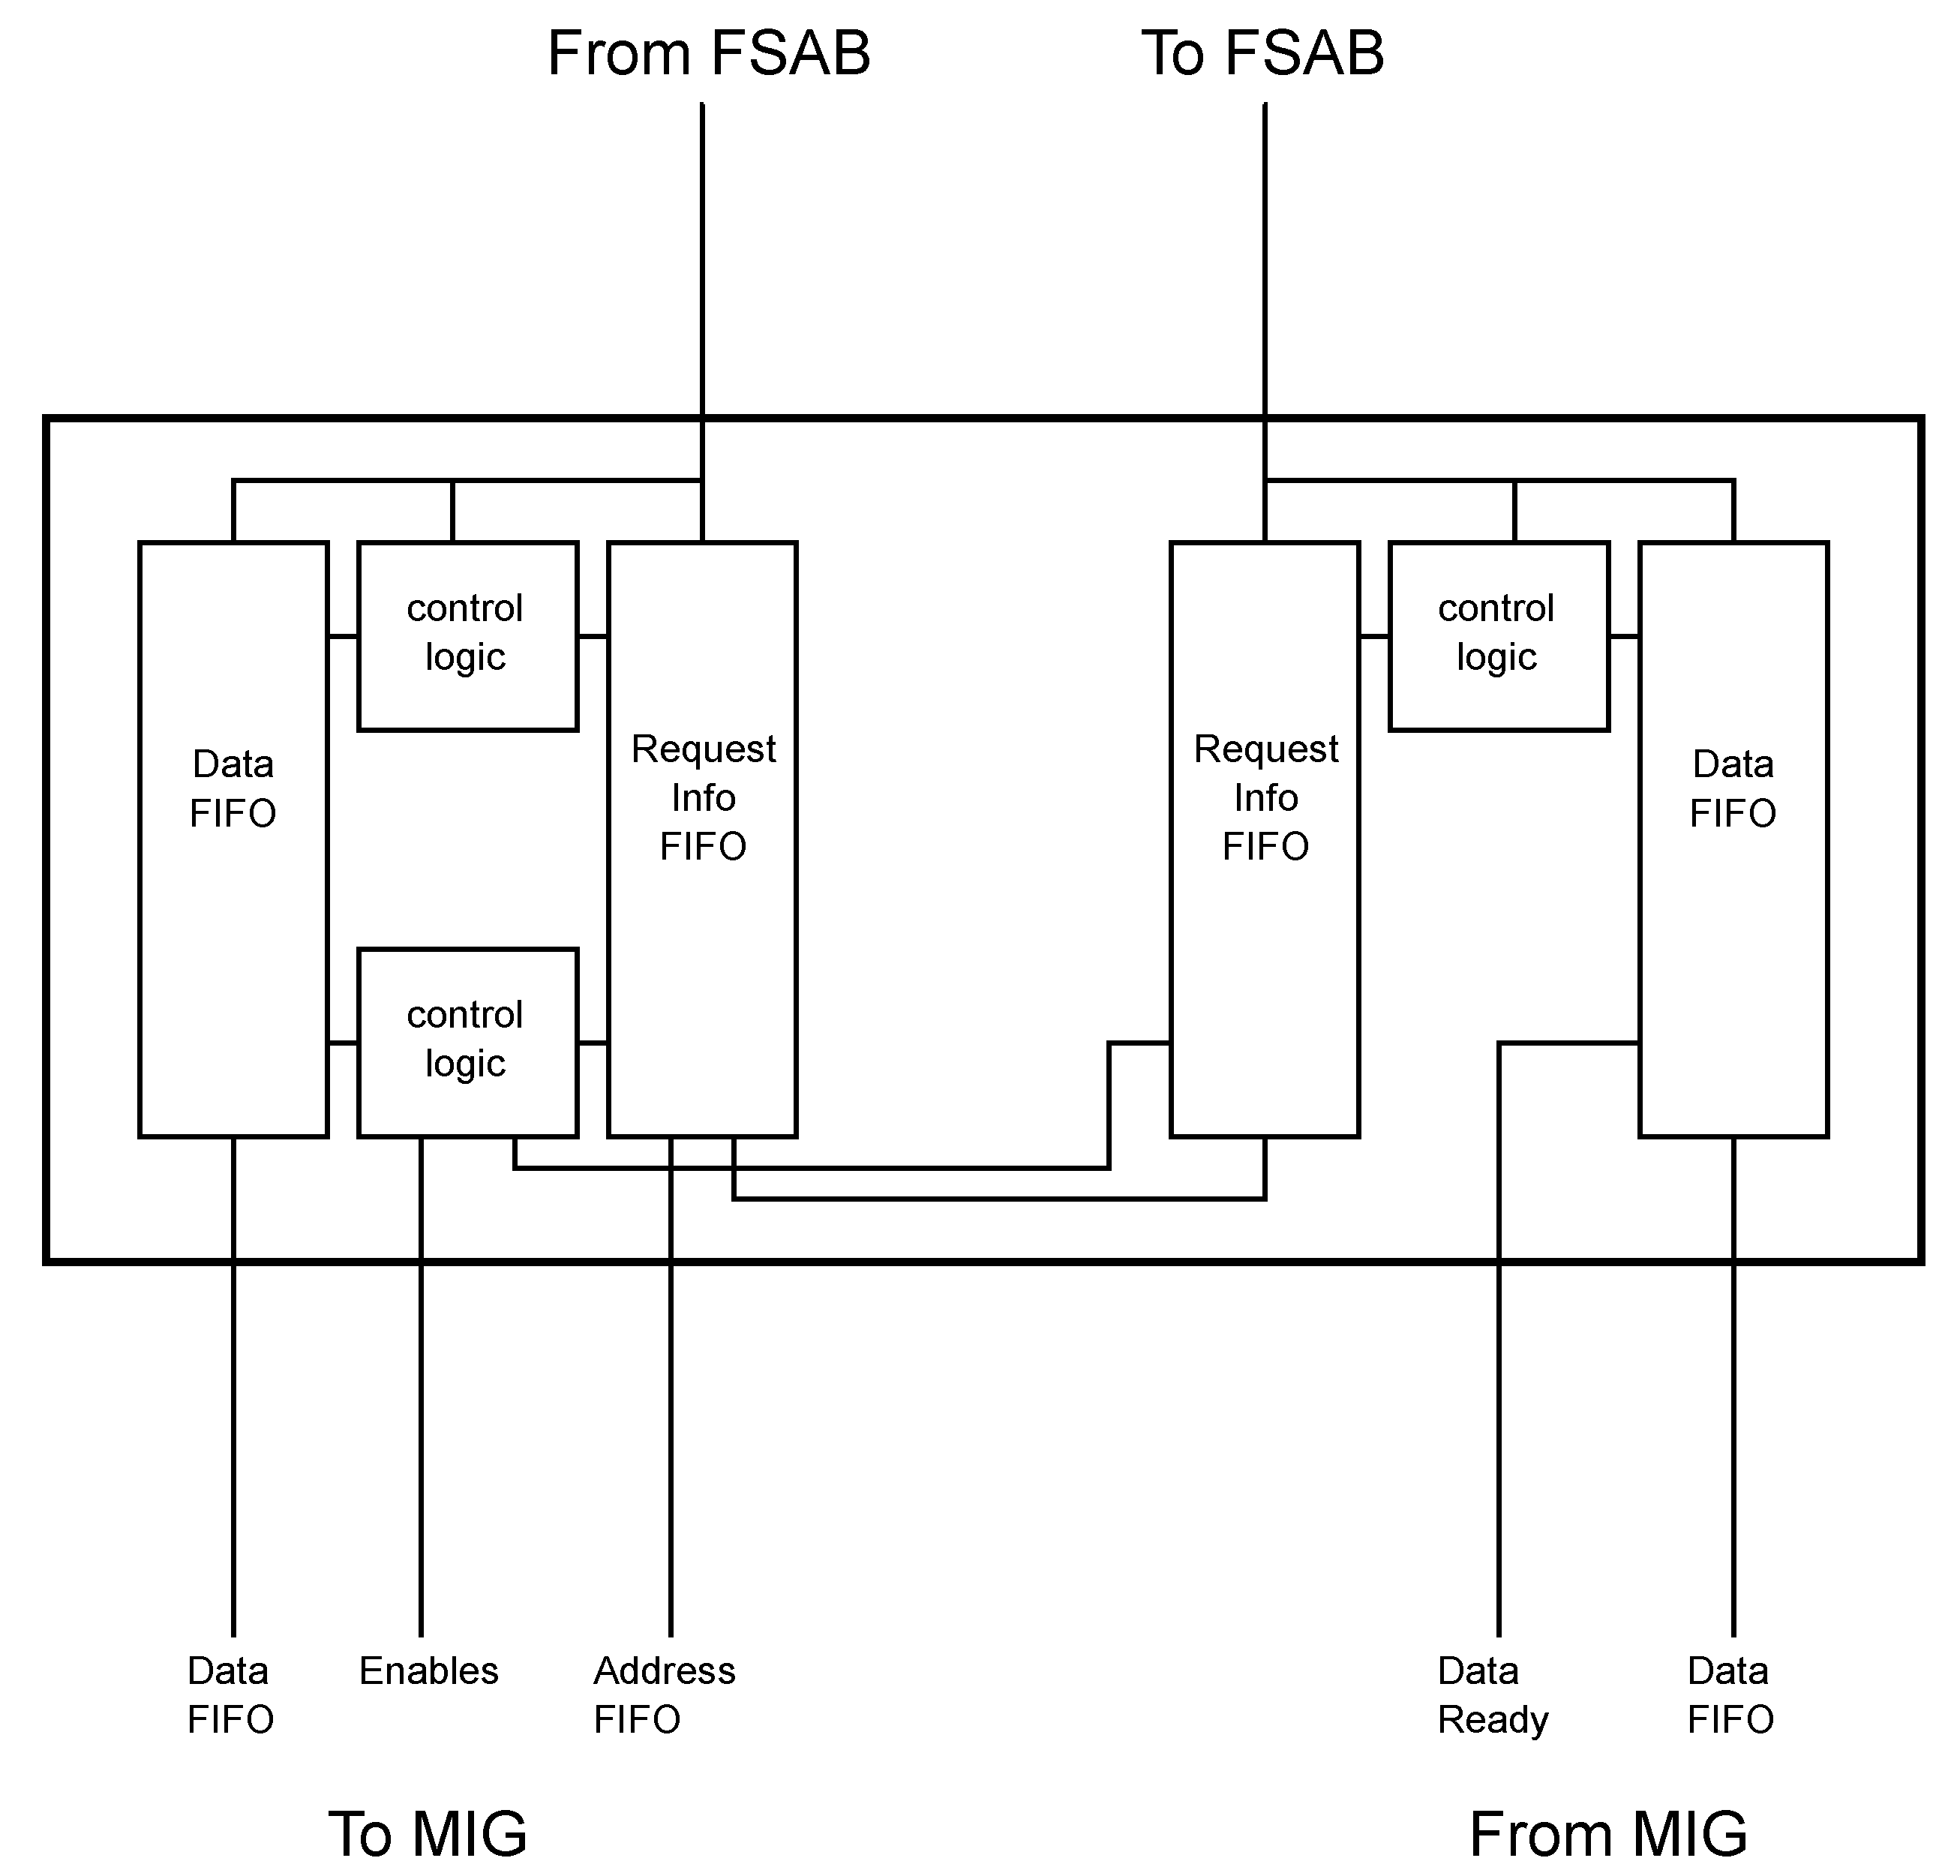
\includegraphics[width=0.85\textwidth]{FSABMemory.pdf}
  \caption{Internals of the memory controller.} \label{fig:fsabmemory}
\end{figure}


The memory controller is best described by tracing the lifetime of a request
as it is made on the FSAB, passes through the memory controller and MIG, and
is returned to the requesting device. At the first packet of the request,
the device identifiers, address, and length are stored in the request info
FIFO. If the request is a write request, the controller reads packets of
data into the data FIFO until the entire request is stored in the FIFO. Each
entry in the data FIFO is two packets wide; the MIG requires data to be
double-wide to facilitate DDR memory. If a write request is not aligned, the
controller inserts a packet's worth of masked data at the front of the
request.

Once the entire transaction has been stored in the FIFOs, the controller
sends it to the MIG. The MIG performs burst operations of a standard length
(in the current implementation, 8 words of 64 bits each; because the memory
is DDR, it takes four clock cycles to transmit or receive a burst). The
request begins with a write to the MIG address and command FIFOs. On a write
request, the first write to the data and mask FIFOs is in the same clock
cycle, and the rest of the burst follows on consecutive cycles. If the
actual request is shorter than the burst length, masked data is written for
the remainder of the burst. On a read request, the device identifier and
request length are stored in the output request info FIFO.

On a read request, some time after sending the request to the MIG, the MIG
will send data back. This data is read into the output data FIFO. When the
data FIFO becomes not empty, the controller reads the device identifier and
length from the request FIFO and the first row from the data FIFO. Data is
returned to the device, with reads from the double-width FIFO every two
packets, until the full length has been transmitted.

\subsection{Known Bugs}

\begin{itemize}
\item{Reads not aligned to whatever boundary the MIG wants are incorrect
(the address is not stored in the output-side request info FIFO, so the
output side has no way to know that the first data the MIG returns is not
the requested data).}
\item{Reads not of the full burst length may mess everything up, since I
don't think we discard the rest of the data the MIG returns in its burst.}
\end{itemize}

\section{Synchronization Mechanisms}

\label{sec:sync}

Within virtexsquared, there are two ``utility'' modules that are commonly
used for synchronizing across clock domain boundaries -- the CSR
synchronizers, and the async FIFO.

\subsection{CSR Synchronizers}

\label{sec:csrasync}

\subsubsection{Motivation and Design Overview}

Since the virtexsquared system has many peripherals on different clock
domains, it only makes sense to have a unified mechanism of synchronizing
SPAM accesses between those domains and the core. Synchronization logic is
not only difficult to write, but it is also difficult to verify the
correctness of; to that end, by encapsulating the synchronization mechanisms
as much as possible, we stand a much better chance of writing correct code.
The Configuration Space Register (CSR) synchronizers are one of two primary
mechanisms for synchronization; for the other, see the AsyncFifo
implementation in section \ref{sec:fifo}.

It was decided early on that CSRAsyncRead and CSRAsyncWrite should be two
different modules, and that there should be no CSRAsyncReadWrite module.
Since the registers that the CSR interfaces mirror are usually primarily
controlled by the peripheral's internal logic, holding register state inside
a ReadWrite module would result in vastly unnecessary complexity, and would
substantially obscure the intent of the logic in the peripheral. (Indeed,
often the resulting state of the register after a write operation is not the
same as the data that was written.)

The CSRAsyncRead and CSRAsyncWrite modules are designed to closely mirror
the SPAM bus protocol; for many uses, the CPU side (on the cclk domain) can
be directly or'ed in on the SPAM bus to implement a peripheral's CSR space.
The target side (on the tclk domain) was designed to produce single cycle
strobes that can be effectively used by a target's internal logic to trigger
updates.

\subsubsection{Interface}

The CSRAsyncRead and CSRAsyncWrite modules are parameterized across the
width of the register that they are synchronizing; the CSRAsyncWrite module
is also parameterized for its reset value.  Both modules have two clock
inputs, and their corresponding negated resets -- \texttt{cclk} is the clock
corresponding to the CPU core that initiates a request, and \texttt{tclk} is
the clock corresponding to the target peripheral.  All ports are suffixed
with the clock domain on which they live (i.e., \texttt{rst\_b\_cclk} and
\texttt{rst\_b\_tclk}).

Both modules have the same core port structure for synchronizing between the
two domains; the only difference in their portlist is in direction on the
data port. The portlist for the read module is as such:

\begin{lstlisting}[basicstyle=\footnotesize,language=Verilog]
input                rd_strobe_cclk;
output [(WIDTH-1):0] rd_data_cclk;
output               rd_wait_cclk;
output               rd_done_strobe_cclk;
 
output               rd_strobe_tclk;
input  [(WIDTH-1):0] rd_data_tclk;
\end{lstlisting}

This provides for a relatively straightforward mechanism for interfacing
with the SPAM bus. For example, the following code for reading a counter was
taken from the blit accelerator:

\begin{lstlisting}[basicstyle=\footnotesize,language=Verilog]
wire [30:0] rd_data_WRDONE;
wire rd_done_strobe_WRDONE;
 
CSRAsyncRead #(.WIDTH(31))
  CSR_WRDONE_READ(/* NOT AUTOINST */
        // Outputs
        .rd_data_cclk      (rd_data_WRDONE),
        .rd_wait_cclk      (),
        .rd_done_strobe_cclk(rd_done_strobe_WRDONE),
        .rd_strobe_tclk    (),
        // Inputs
        .cclk              (cclk),
        .tclk              (fsabi_clk),
        .rst_b_cclk        (cclk_rst_b),
        .rst_b_tclk        (fsabi_rst_b),
        .rd_strobe_cclk    (rd_decode &&
                            (spamo_addr[4:0] == 5'b10100)),
        .rd_data_tclk      (wrdone[30:0]));
 
assign accel_blit__spami_busy_b =
  /* ... */ | rd_done_strobe_WRDONE;
assign accel_blit__spami_data =
  {32{rd_done_strobe_WRDONE}} & {1'b0, rd_data_WRDONE};
\end{lstlisting}

The instantiation mechanism is somewhat bulky, but it is certainly better
than reimplementing the synchronizer each time! Future work may be possible
to extend verilog-mode to be able to automatically instantiate CSR
synchronizers.

\subsubsection{Implementation}

The synchronizers are based around sound two-flop principles for
synchronizing between clock domains. In order to transmit a value between
the two clock domains, the ``hold-and-sample'' technique is used; once a
flag is seen indicating that new data is ready to be transferred, the
synchronizers wait a cycle before sampling the data and transmitting it to
the recipient clock domain. Building on this principle, the synchronizers
can be trivially implemented with a small amount of internal state to
generate strobes and output data.

All internal signals are named according to the clock domain on which they
live; signals named \texttt{...\_tclk} are on the target clock, and signals
named \texttt{...\_cclk} are on the core clock.  To synchronize a signal,
the progression of naming \texttt{foosig\_cclk}, \texttt{foosig\_cclk\_s1},
and \texttt{foosig\_cclk\_tclk} is used to represent the signal after no
flops, one flop, and two flops, respectively.

\subsection{Synchronous FIFO}

\label{sec:syncfifo}

Although the synchronous FIFO is not strictly a clock synchronization
mechanism, it is presented in this section as a means to understanding the
asynchronous FIFO, and since it is a fundamental building block of the
system.

\subsubsection{Motivation}

There are a number of reasons to have a packaged-up FIFO utility. One is
cleanliness and readability of code; an instantiation of a FIFO module is
immediately apparent to a reader, while an implementation mixed in with
other code is less so. Another reason for the Fifo module is the reduction
of opportunities for bugs; every implementations of FIFOs scattered through
the RTL is another opportunity for a mistake to appear, costing valuable
debug time (around 20 minutes per synthesis run).

\subsubsection{Implementation}

The Fifo module is implemented as a block RAM with read and write pointers.
Both pointers are initialize to zero; after a read or write, the appropriate
pointer increments. If the pointers are equal, the FIFO is empty. (Each
pointer is one bit wider than required to index into the RAM so that a full
FIFO does not appear identical to an empty FIFO.)

\subsubsection{Implementation: Parameters}

\begin{itemize}
\item{\textbf{DEPTH}: how many entries the FIFO can store}
\item{\textbf{WIDTH}: how many bits each entry has, and the width of the input and
output data ports}
\item{\textbf{ALMOST}: how few entries away from full or empty the FIFO must be to be
considered almost full or almost empty}
\end{itemize}

\subsubsection{Implementation: Portlist}
\begin{lstlisting}[basicstyle=\footnotesize,language=Verilog]
input clk;
input rst_b;
 
input wr_en;
input rd_en;
input [WIDTH-1:0] wr_dat;
 
output [WIDTH-1:0] rd_dat;
output empty;
output full;
output [`ADDR_WIDTH:0] available;
output afull;
output aempty;
\end{lstlisting}

At a positive clock edge, when wr\_en is high, the data at wr\_dat is stored
in the FIFO, and when rd\_en is high, the next entry in the FIFO is presented
at rd\_dat.

Interesting outputs:
\begin{itemize}
\item{\textbf{empty}: is high when the FIFO is empty}
\item{\textbf{full}: is high when the FIFO is full}
\item{\textbf{afull}: is high when there are ALMOST or fewer empty spaces left in the
FIFO. \footnote{\Huge{\textbf{I'M ALMOST FULL!!!}}} }
\item{\textbf{aempty}: is high when there are ALMOST or fewer entries in the FIFO}
\item{\textbf{available}: the number of entries in the FIFO; the width of this port is
log${}_2$ DEPTH + 1}
\end{itemize}

\subsection{Asynchronous FIFO}

\label{sec:fifo}

\subsubsection{Motivation}

As with a simple FIFO, there are a number of motivations for a packaged
cross-clock-domain FIFO utility: code reuse, clarity, and reduction of bugs.
This last motivation carries significant additional weight for a
cross-clock-domain FIFO: hardware crossing multiple clock domains is tricky,
so the less of it that needs to be written, the better.

\subsubsection{Implementation}

The core fifo implementation is similar to that to that of the Fifo module
(see section \ref{sec:syncfifo}): a block RAM with read and write
pointers.  Reads from and writes to the block RAM occur on the different
clock domains.  To accommodate empty and full outputs, the pointers must be
converted into grey code and passed across the clock domain boundary.  The
empty output is on the read clock domain (so that the module using the FIFO
can avoid reading when empty), and the full output is on the write clock
domain (so that the module using the FIFO can avoid writing when full).  To
accomplish this, both pointers are converted to grey code, passed through a
register, and passed across the clock domain boundary, and passed through
two more registers (to avoid metastability).

Because of the delay associated with crossing the clock domain boundary, it
is possible that the module may incorrectly indicate an empty or full FIFO. 
However, it will be incorrect in the other direction (with a false
negative).  This is guaranteed for the empty output because it is the write
index which is late: there can be \textit{more} data in the FIFO than the
reader knows about, but since the read index is not delayed, there is never
\textit{less}.  (Similar reasoning holds for the full output.)

\subsubsection{Implementation: Parameters}

\begin{itemize}
\item{\textbf{DEPTH}: how many entries the FIFO can store}
\item{\textbf{WIDTH}: how many bits each entry has, and the width of the input and
output data ports}
\end{itemize}

\subsubsection{Implementation: Portlist}
\begin{lstlisting}[basicstyle=\footnotesize,language=Verilog]
input iclk;
input oclk;
input iclk_rst_b;
input oclk_rst_b;
 
input wr_en;
input rd_en;
input [WIDTH-1:0] wr_dat;
 
output [WIDTH-1:0] rd_dat;
output empty;
output full;
\end{lstlisting}

\section{Simple DMA Read Controller}
\label{sec:dmac}

The Simple DMA (Direct Memory Access) Read Controller provides a FIFO-like
interface for a target peripheral to read from memory.

\subsection{Motivation}

Since many devices require memory read access in a linear pattern, it only
made sense to support such access pattern in a simple way.

\subsection{Conceptual Overview}

After providing a start address, length, and a trigger command through the
SPAM bus (see section \ref{sec:spam}), data\_ready will be asserted high and
the master will be able to get the next 8 bytes of data one cycle after
request is asserted high as long as the FIFO (queue) is not empty (no
underflow).  Once the DMA is done reading through the entire length, it may
be triggered again to read from a new start address and different length.

\subsection{Design Overview}

\subsubsection{Portlist}

Simple DMA Read Controller has the following ports that the master should
not directly interact with:

\begin{itemize}
\item{the default FSAB portlist (prefixed by dmac\_\_ for outbound)}
\item{SPAM portlist (prefixed by dmac\_\_)}
\end{itemize}

For the master, it has the following ports:

\begin{lstlisting}[basicstyle=\footnotesize,language=Verilog]
input request; 
input target_clk; /* clk that the master is running in */
input target_rst_b;
output [63:0] data; /* 8 bytes of new data */
output data_ready;
output fifo_empty; 
/* asserted when the fifo is empty. This may be the case when there is an
 * underflow or when the DMA didn't start reading */
\end{lstlisting}

\subsubsection{Parameters}

\begin{lstlisting}[basicstyle=\footnotesize,language=Verilog]
parameter FIFO_DEPTH = 128; /* must be a power of 2 */
parameter FIFO_HI = clog2(FIFO_DEPTH) - 2;
parameter FSAB_DID = 4'hF;
parameter FSAB_SUBDID = 4'hF;
parameter SPAM_DID = 4'hx;
parameter SPAM_ADDRPFX = 24'h000000;
parameter SPAM_ADDRMASK = 24'hFFFFE0;
parameter DEFAULT_ADDR = 31'h00000000;
parameter DEFAULT_LEN = 31'h00000000;
\end{lstlisting}

The parameters are defined as follows:

\begin{itemize}
\item{\textbf{FIFO\_DEPTH}: Depth of the internal FIFO. DMA Controller will
try to keep this FIFO as full as possible. This value must be a power of 2
and 8 or greater to be functional.}
\item{\textbf{FIFO\_HI}: Highest bit needed to represent FIFO\_DEPTH space.
(log${}_2$(FIFO\_DEPTH) - 2) if FIFO\_DEPTH is power of 2.}
\item{\textbf{FSAB\_DID}: FSAB device id of the master. (if the master
doesn't have one, give the master one by setting it in
\texttt{rtl/fsab/fsab\_defines.vh})}
\item{\textbf{FSAB\_SUBDID}: FSAB sub device id of the master. (if the
master doesn't have one, give the master one by setting it in
\texttt{rtl/fsab/fsab\_defines.vh})}
\item{\textbf{SPAM\_DID}: SPAM device id of the master. (if the master
doesn't have one, give the master one by setting it in
\texttt{rtl/spam/spam\_defines.vh})}

\item{\textbf{SPAM\_ADDRPFX} and \textbf{SPAM\_ADDRMASK}: To write/read from
the SPAM bus, it must be the case that \texttt{((spamo\_addr \& SPAM\_ADDRMASK) ==
SPAM\_ADDRPFX)}.  (Note: Always set the last 5 bits of the SPAM\_ADDRMASK to
0.)}

\item{\textbf{DEFAULT\_ADDR}: Default starting address for the DMA.}

\item{\textbf{DEFAULT\_LEN}: Default length that the DMA will read. The DMA will
provide values starting from address up to the length.}

\end{itemize}

\subsubsection{Config Registers (SPAM)}

The following values come from \texttt{rtl/fsab/dma\_config\_defines.vh};
these addresses correspond to the last 5 bits that the spamo\_addr needs to
be set to refer to these registers.

\begin{lstlisting}[basicstyle=\footnotesize,language=Verilog]
parameter NEXT_START_REG_ADDR = 5'h000;
parameter NEXT_LEN_REG_ADDR = 5'h004;
parameter COMMAND_REG_ADDR = 5'h008;
parameter FIFO_BYTES_READ_REG_ADDR = 5'h00c;
parameter TOTAL_BYTES_DELIVERED_REG_ADDR = 5'h010;
parameter CURR_START_REG_ADDR = 5'h014; 

parameter DMA_STOP = 2'b00;
parameter DMA_TRIGGER_ONCE = 2'b01;
parameter DMA_AUTOTRIGGER = 2'b10;
\end{lstlisting}

The registers are defined as follows:

\begin{itemize}
\item{\textbf{NEXT\_START\_REG (write only)}: sets the starting address of
the DMA for the \textbf{next time} it is triggered.}

\item{\textbf{NEXT\_LEN\_REG (write only)}: sets the length that the DMA has
to read for the \textbf{next time} it is triggered.}

\item{\textbf{COMMAND\_REG (write only)}: sets the next command for the DMA
engine to execute, from one of:}
\begin{itemize}
\item{\textbf{DMA\_STOP}: DMA does not trigger again.}
\item{\textbf{DMA\_TRIGGER\_ONCE}: Triggers the DMA once.}
\item{\textbf{DMA\_AUTOTRIGGER}: Everytime, the DMA is done reading, it is
triggered again.}
\end{itemize}

\item{\textbf{FIFO\_BYTES\_READ\_REG (read only)}: the number of bytes that
the \textit{internal FIFO} has read so far since it was last triggered.}

\item{\textbf{TOTAL\_BYTES\_DELIVERED\_REG (read only)}: the total number of
bytes that was delivered to the master since the \textit{last reset}. (note:
it is not ``last triggered'')}

\item{\textbf{CURR\_START\_REG (read only)}: the address that the DMA
started reading from. (It provides the value of NEXT\_START\_REG before it was
triggered)}

\end{itemize}

\subsubsection{Implementation}

The internal queue for DMA is represented in the following way:

\begin{lstlisting}[basicstyle=\footnotesize,language=Verilog]
reg [FSAB_DATA_HI:0] fifo [(FIFO_DEPTH-1):0];
 
/* Clock domain: fsabi_clk */
reg [FIFO_HI:0] fifo_wpos;
 
/* Clock domain: target_clk */
reg [FIFO_HI+1:0] curr_fifo_length;
reg [FIFO_HI:0] fifo_rpos;
\end{lstlisting}

While the DMA is triggered, it attempts to obtain data in 64 byte blocks
using FSAB as long as there is space in the queue for it. When the request
for 64 byte block is sent, these data will come 8 bytes at a time. Whenever,
a value arrives, the value is stored in the fifo but \textbf{only} fifo\_wpos changes
values. Once all 64 bytes arrive, a completion message gets synchronized
from fsabi\_clk domain to target\_clk domain so that curr\_fifo\_length can be
updated. fifo\_rpos is used to read values from the fifo to provide data to
the master.

\subsection{Users}

The Simple DMA Read Controller is used by:

\begin{itemize}
\item{Framebuffer (see section \ref{sec:framebuffer})}
\item{Audio (see section \ref{sec:audio})}
\end{itemize}

\section{Framebuffer}
\label{sec:framebuffer}

The framebuffer provides pixeldata to the DVI to be displayed on the screen.

\subsection{Conceptual Overview}

Framebuffer uses the Simple DMA Read Controller (see section \ref{sec:dmac})
to obtain pixel data to be displayed and uses SyncGen to figure out whether
the value needs to be sent for display.

Notes:

\begin{itemize}
\item{Four bytes contain data for one pixel.}
\item{Each primary color uses one byte (RGB) and occupies the first 3
bytes.}
\item{The last byte is thrown away.}
\item{(Be aware of little endianness while programming...)}
\end{itemize}

\subsection{Framebuffer DMA configuration}

These can be accessed through 0x820000$<$Register Addr$>$

Some relevant addresses for the framebuffer are:

\begin{itemize}
\item{\textbf{0x82000000 (write only)}: Framebuffer DMA start address (for setting buffer
locations)}
\item{\textbf{0x82000004}: Framebuffer length}
\item{\textbf{0x82000014 (read only)}: Start address of the buffer currently being read by
the DMA (needed for triple buffering).}
\end{itemize}

\subsection{Example Usage}

The Framebuffer is used by the multibuf library (see section
\ref{sec:multibuf}).

\section{Audio}

\label{sec:audio}

The audio module streams sample frames to the AC'97 codec to generate sound.

\subsection{Motivation}

Our application required an audio and we only needed to make simple
modifications to the SimpleDMAReadController (see section \ref{sec:dmac})
for it to be usable for producing audio from a range of address.  We also
had ACLink and AC97Conf that are from our 2nd lab.

\subsection{Implementation}

Audio module contains few improvements from our AC97 base code:

\begin{itemize}
\item{AudioGen is replaced with DMA to fetch audio data from DRAM}
\item{Some additional logic has been added because DMA provides data in
chunks of 8 bytes.}
\item{AC97 configuration can be controlled through the SPAM bus.}
\end{itemize}

\subsection{Audio Configuration Registers}

We have chosen these addresses to not conflict with the DMA configuration
registers.  The registers are:

\begin{itemize}
\item{\textbf{0x84000100 (write only)}: Master Volume}
\item{\textbf{0x84000104 (write only)}: Microphone Volume}
\item{\textbf{0x84000108 (write only)}: Line In Volume}
\item{\textbf{0x8400010C (write only)}: Audio CD Volume}
\item{\textbf{0x84000110 (write only)}: Audio PCM Volume}
\item{\textbf{0x84000114 (write only)}: Audio Recording Select}
\item{\textbf{0x84000118 (write only)}: Audio Recording Gain}
\end{itemize}

\subsection{To do}

\begin{itemize}
\item{Need a way to stop/pause a playing audio.}
\end{itemize}

\section{PS2}
\label{sec:ps2}

The PS2 module obtains PS2 keyboard scancode data and stores each value into
a fifo such that the value could be obtained one at a time through the SPAM
bus.

\subsection{Portlist}

The PS2 module includes the SPAM portlist (see section \ref{sec:spam}),
prefixed by ps2\_\_ on all outbound.

\begin{lstlisting}[basicstyle=\footnotesize,language=Verilog]
input ps2clk;
input ps2data;
\end{lstlisting}

The PS2 module complies with the timings listed in the
\href{http://www.digilentinc.com/Data/Products/NEXYS2/Nexys2_rm.pdf}{Nexys 2
reference manual} on page 8.

\subsection{Implementation Details}

Since the data arrives asynchronously (it is a keyboard input afterall),
ps2clk must first be latched with 2 flip flops to get a stable value.

Then, one would wish to obtain each data by checking the value at the
negative edge. Unfortunately, ps2clk is not a real clock so the method
doesn't work. Instead, the value of ps2clk is checked every positive edge of
the core clock(cclk) and detects the falling edge of ps2clk. This is a valid
method only because the core clock is much faster than the ps2clk.

Once all 11 bits (\{start\_bit, scancode\_data[7:0], odd\_parity\_bit,
stop\_bit\}) are received and odd parity check matches, scancode data is
stored in the queue.

When a request for scancode data is made through the spam bus, if the fifo
is empty, 0xFFFFFFFF is returned. Otherwise, a value is dequeued from the
fifo and returns \{24'h0, scancode\_data\}.

\subsection{Usage}

For an example of usage, see the keyhelp library in section
\ref{sec:keyhelp}.

\subsection{To Do}

\begin{itemize}
\item{Sending data to the keyboard to have Num Lock, Caps Lock, and Scroll
Lock lights flashing when appropriate. (Or change the scancode set of the
keyboard if we want to use 15-410 version of process\_scancode instead)}
\item{The keyboard should still work after being unplugged and replugged
many times.}
\end{itemize}


\section{Timer}

\label{sec:timer}

The timer module provides the number of clock cycles since reset through the
SPAM bus (see section \ref{sec:spam}).

\subsection{Motivation}

As we started writing the game and painted arrows on the screen, we quickly
realized that performance may become an issue. Whenever we made a change to
RTL or our code, we needed a way to measure performance. The number of clock
cycles since reset seemed to be the easiest way to measure this.

\subsection{Portlist}

The Timer module includes the SPAM portlist (see section \ref{sec:spam}),
prefixed by timer\_\_ on all outbound.

\subsection{Usage Example}
\begin{lstlisting}[basicstyle=\footnotesize,language=C]
#include <minilib.h>
int *timer = 0x86000000;
printf("Cycles: %d\r\n", *timer);
\end{lstlisting}

\subsection{To Do}

\begin{itemize}
\item{Have a real timer that returns real time in ms since reset instead of
core clock cycles}
\item{Clock cycle counter overflows too often (approximately every 30
seconds)}
\end{itemize}

\section{Hardware Blit/Clear Accelerators}
\label{sec:accel}

\subsection{Clear Accelerator}

\subsubsection{Motivation}

Whenever we got a new buffer (see the section on multibuf, section
\ref{sec:multibuf}) to start drawing, we always had to clear the screen and
draw things on top of the cleared screen.  This meant that we had to
effectively draw the screen twice.  We figured that clearing the screen in
hardware is relatively easy and give big performance boost.  This also has
many uses because it is effectively a memset accelerator assuming that start
address is 64-byte aligned and length is 8-byte aligned.

\subsubsection{Implementation}

Implementation is similar to the Simple DMA Read Controller without the
queue. Every time the clear accelerator gets control of the FSAB bus, it
writes up to 64 bytes.

\subsubsection{Implementation: Portlist}

The clear accelerator's port list consists simply of the SPAM portlist
(prefixed by accel\_ for the outbound), and the FSAB portlist (prefixed by
accel\_ for the outbound).

\subsubsection{Implementation: Configuration Space Registers}

\begin{itemize}
\item{\textbf{4'b0000 (write only)}: 4 byte data that every value inside
[start\_address, start\_address+num\_packets*8) need to be set to.  Must be
64-byte aligned.}
\item{\textbf{4'b0100 (write only)}: start address (start\_address)}
\item{\textbf{4'b1000 (read/write)}: number of FSAB packets (num\_packets) - each fsab
packet is 8 bytes since FSAB\_DATA\_HI = 63 (64 bit transaction at a time)}
\end{itemize}

AccelClear begins clearing when the number of FSAB packets is set to a value
greater than 0.

\subsubsection{Usage}

See the section on the accel library, section \ref{sec:accel_lib}.

\subsection{Blit Accelerator}

\subsubsection{Motivation}

When we realized that our application is not drawing fast enough ($\le$ 30
frames per second) even after clear accelerator and triple buffering, we
realized that we needed to make another improvement.

We had two options:
\begin{itemize}
\item{Rewrite the blitter we had in software in assembly. We believed that
this would give us a performance boost because the assembly code that the
compiler gave just didn't seem very good.}
\item{Write a \texttt{bitblt} (``blit'') accelerator in hardware.}
\end{itemize}

We went with the blit accelerator in hardware because we were confident that
a blit accelerator would give a big performance boost.

\subsubsection{Implementation}

There are 3 stages:
\begin{enumerate}
\item{Read 64 bytes from current read address and increment the current read
address by 64.}
\item{Write those 64 bytes to the current write address.}
\item{Increment write address by 64 if a row hasn't been completed or make
it point to the next row.}
\end{enumerate}

\subsubsection{Implementation: Portlist}

The blit accelerator's port list consists simply of the SPAM portlist
(prefixed by accel\_ for the outbound), and the FSAB portlist (prefixed by
accel\_ for the outbound).

\subsubsection{Implementation: Configuration Space Registers}

\begin{itemize}
\item{\textbf{5'b00000 (write only)}: read start address (must be 64-byte
aligned)}
\item{\textbf{5'b00100 (write only)}: read length (in 64-byte packets)}
\item{\textbf{5'b01000 (write only)}: write start address}
\item{\textbf{5'b01100 (write only)}: write row length (in 64-byte packets)}
\item{\textbf{5'b10000 (write only)}: write row stride (in bytes)}
\item{\textbf{5'b10100 (read/write)}: = 64-byte packets written}
\end{itemize}

The blit accelerator begins blitting when read length is set to a value greater
than 0.

\subsubsection{Usage}

See the section on the accel library, section \ref{sec:accel_lib}.

\section{SystemACE Interface}

\subsection{Motivation and Design Constraints}
At some point during the development process, it was decided that using the
linear StrataFlash, as done on the initial AC'97 demo project, would be
insufficient; the size of the flash is insufficient to store substantial
quantities of music, and reprogramming new data onto the flash requires a
relatively lengthy process over JTAG. It was decided, then, that the
SystemACE's CompactFlash card interface should be used to load code and data
into the running system.

The SystemACE provides a very usable microcontroller interface to its
internal registers; these registers can be used to command the CompactFlash
card, and interrogate other aspects of the system's state. It was decided
that the easiest mechanism to gain access to these registers - and hence the
CompactFlash card - was to add a ``glue'' interface between the MPU pins and
the SPAM bus. If additional performance was needed later from CompactFlash
requests, then FSAB DMA could be added; but the first priority was to gain a
working mechanism to access the CompactFlash, with the simplest hardware
possible.

\subsection{Interface}

The SystemACE module provides a device on the SPAM bus with DID 4'h3 (i.e.,
with base address 0x83000000). Registers are linearly mapped into the SPAM
address space on dword (four-byte) boundaries; that is to say, A$<0>$ on the
SystemACE is wired to A$<2>$ on the SPAM, and so on up. A complete register
mapping of the SystemACE interface can be found on Xilinx's site, in
\href{http://www.xilinx.com/support/documentation/data_sheets/ds080.pdf}{DS080:
SystemACE CompactFlash Solution}. Since all 16 data pins are connected
through on the XUPV5, the device can be used in word-wide mode (i.e., with
0x1 written to address 0x83000000).

\subsection{Implementation}

A very similar synchronization mechanism to that used in the
CSRAsyncRead/Write blocks (see section \ref{sec:csrasync}) is employed to
synchronize addresses along with data between the CPU clock and the
SystemACE clock domain.  However, some changes are noted; for instance,
since CSRAsyncRead is not reading directly from a register, it must also
wait for a response to come back from the SystemACE before it acknowledges
the request (and sends the data back) to the CPU clock domain.  Similarly,
since the external bus protocol for the SystemACE is not quite as simple as
a write enable on a register, or a read from a multiplexed register;
instead, the external bus lines must be driven in a certain order.  This is
implemented in a state machine with seven states that ensure that setup and
hold times are all met.

Appropriate tristate gating to the outside world is enforced using a raw
IOBUF instantiation. One possible alternative coding style for this is to
use an inout reg that can be set to z; tests determined that although
somethings Xilinx tools correctly synthesize this, other times the tools
fail to synthesize this as a tristateable output. Manually invoking the
IOBUF primitive forces the tools to generate the correct routing for the
tristate enable.

\subsection{Software}

Software support for the SystemACE controller is provided by the
\texttt{sysace} and \texttt{fat16} libraries in \texttt{sw/lib}.  The
primary external interfaces to sysace are \texttt{sysace\_init()} and
\texttt{sysace\_readsec()}; other functions are intended as internal
mechanisms exported only because they are named processes in the SystemACE
user's guide.

The \texttt{fat16} library is best investigated by example;
\texttt{sw/boot1} provides a good example of using the FAT16 driver to list
the contents of the root directory, and to open and load the application
code ELF image.

\chapter{Software Design}

In this part, we mention salient libraries located in \texttt{sw/lib} that we 
designed to abstract some of the details of the hardware.

\section{Multibuf Library}

\label{sec:multibuf}

Multibuf library implements \href{http://en.wikipedia.org/wiki/Multiple_buffering#Triple_buffering}{triple buffering} for screen display 

\subsection{Motivation}

Originally, we had double buffering but performance was an issue. In double buffering, after the framebuffer start address has switched, the code couldn't continue writing to the new buffer because the dma may not have started reading from the new address yet. This caused a notable choppiness of the arrows going up the screen in Stepmania. After measuring the time this took with Timer module (see section \ref{sec:timer}), we decided to implement triple buffering. 

\subsection{Implementation Details}

multibuf\_init allocates three arrays of size (width*height*4+64) bytes, aligns it to 64 bytes (because of the warning in DMA controller(See section \ref{sec:dmac}) ), and calls multibuf\_flip to provide a new buffer.

multibuf\_flip sets the frame buffer DMA's start\_addr (0x82000000) to the buffer that is currently writing and provides a new buffer that the DMA is currently not reading (can be read from 0x82000014). Since only two buffers could be used in the worst case, there is always a new buffer that could be returned immediately.

\subsection{Example Usage}

\begin{lstlisting}[basicstyle=\footnotesize,language=C]
   multibuf_t multibuf;
   int* buf;
   buf = multibuf_init(&multibuf, 640, 480); /* 640 by 480 screen */
   /* fill the buffer of size 640*480 ints where the last 3 bytes are BGR (thanks to little endianness)
   and whatever you feel like in the first byte */
   buf = multibuf_flip(&multibuf); 
   /* now the buffer you wrote to the buffer will be displayed on the screen and you 
      can write more stuff to the new buffer */
   buf = multibuf_flip(&multibuf);
\end{lstlisting}

\section{Keyhelp Library}

\label{sec:keyhelp}

Keyhelp library contains a function to process scancode and other helper macros to read keyboard input

\subsection{Motivation}

After implementing the RTL for obtaining scancode from PS/2, it became apparent that we need a function like process\_scancode from 15-410 kernel. We wanted to use the process\_scancode code that they had but the process\_scancode that 15-410 kernel has implemented is for set 1 scancodes and the default scancodes we got when we plugged in our keyboard was set 2. That meant that we either had to modify our RTL to support changing sets or had to write a new process\_scancode function. We ended up writing a new process\_scancode because writing more RTL is more difficult than writing more C code. (See \href{http://en.wikipedia.org/wiki/Scancode}{scancode} for differences) 

\subsection{Implementation}

The implementation of process\_scancode is very similar to the one from 15-410 except it is for scancode set 2 and doesn't implement all the keys. It contains an internal state machine to keep track of the current state of the keyboard and returns a value of type kh\_type that could be used with some of the macros from keyhelp.h as shown in example usage.

\subsection{Example Usage}

\begin{lstlisting}[basicstyle=\footnotesize,language=C]
   #include "keyhelp.h"
 
   volatile unsigned int* scancodeaddr = 0x85000000;
   unsigned int scancode;
   kh_type k;
   char new_char;
 
   while ((scancode = *scancodeaddr) != 0xffffffff) {
      k = process_scancode(scancode);
      if (KH_HAS_CHAR(k)) {
         new_char = KH_GET_CHAR(k);
         if (!KH_IS_RELEASING(k)) {
            switch (new_char) {
               case 'z': /* insert code here */
               case 'a': /* insert code here, etc. */ 
               /* etc. etc. */
            }
         }
 
      }
   }
\end{lstlisting}

\section{Accelerator Library}

\label{sec:accel_lib}

Uses hardware accelerator (See section \ref{sec:accel}) to perform acceleration of clearing the framebuffer and bliting images onto the screen.

\subsection{Motivation}

See section \ref{sec:accel}

\subsection{accel\_fill}

(variable names are bolded)

accel\_fill(unsigned int* \textbf{base}, unsigned int \textbf{value}, unsigned int \textbf{words})

Writes \textbf{value} for the next \textbf{words} words starting from \textbf{base}.

\subsubsection{Implementation}

This function is implemented by setting the corresponding config registers of AccelClear (setting length last) and spin waiting until clearing is complete. By spin waiting, Cache does not eat up memory bandwidth and guarantees that bliting is complete when the function completes.

\subsection{accel\_blit}

(variable names are bolded)

accel\_blit(unsigned int* \textbf{base}, unsigned int* \textbf{src}, unsigned int \textbf{w},
            unsigned int \textbf{h})

Copies an image of size \textbf{w} by \textbf{h} represented in \textbf{src} to \textbf{dest} 
(framebuffer) assuming that the screen is 640 pixels wide.

\subsubsection{Implementation}

This function is implemented by setting the corresponding config registers of AccelBlit (setting read length last) and spin waiting until bliting is complete. By spin waiting, Cache does not eat up memory bandwidth and guarantees that bliting is complete when the function completes. 

\section{Audio Library}
\label{sec:libaudio}

Contains various audio helper functions that are implemented with the help of audio module.

void audio\_master\_volume\_set(char \textbf{mute}, char \textbf{left}, char \textbf{right}):

\begin{itemize}
\item{\textbf{mute}: Volume is not muted if 0. Muted otherwise.}
\item{\textbf{left}, \textbf{right}: Sets the volume of left and right speakers.}
\end{itemize}

void audio\_play(void* \textbf{location}, int \textbf{length}, int \textbf{mode}):

\begin{itemize}
\item{\textbf{location}: start location of the audio. (may need to be 64-byte aligned)}
\item{\textbf{length}: length of the audio in bytes. The function will truncate the last 8 bits.}
\item{\textbf{mode}: 0 = stop, 1 = play once, 2 = play repeatedly}
\end{itemize}

void audio\_stop():

int audio\_samples\_played():

int is\_audio\_done(int len): checks whether the audio module finished playing the audio given its length.

\chapter{Miscellaneous System Notes}

In this part, we describe other portions of the system that do not easily
fit as being called either hardware or software, but that still merit
discussion.

\section{virtexsquared Boot Sequence}
\label{sec:boot}

Since the sequence of steps that virtexsquared takes to boot is somewhat
unlike a modern x86 PC, it is worth discussing in brief. Specifically, in
order to boot, control of the system first starts with the SystemACE, is
passed to the preloader, then to boot0, then boot1, and then finally to
application code.

\subsection{SystemACE}

When the board is first powered on, there is no configuration loaded on the
FPGA. In order to get the virtexsquared system running at all, the
configuration must be somehow loaded. If the CompactFlash card is inserted
(and contains the BOOT.ACE file generated from the bitstream), then the
Xilinx SystemACE CompactFlash controller on the board will begin programming
the FPGA over the configuration JTAG interface; this procedure takes about a
second and a half. If CompactFlash FPGA programming fails, then the red LED
on the board will either blink or illuminate statically.

The SystemACE can also be removed from this stage of boot by programming the
board using the external JTAG connector; this is useful when debugging the
design using ChipScope.

When the FPGA is programmed, the internal circuitry begins a post-reset
sequence.

\subsection{Preloader}

Once the FPGA has been configured, the PLLs and DCMs have locked, and the
DRAM PHY has self-calibrated, the preloader is taken out of reset, and
begins performing DMA from an internal block RAM into the very beginning of
DRAM (address 0x0). The preloader DMAs in 8-qword blocks, and transfers a
total of 16 kBytes of data into DRAM. While this occurs, the core is held in
reset using a signal OR'ed in with the normal reset path.

Once the preloader completes, the core is taken out of reset and allowed to
begin operating.

The operation and design behind the preloader is discussed in more detail in
section \ref{sec:preloader}.

\subsection{boot0}

boot0 is the first code that is executed by the ARM core. It begins with a
small fragment of ARM assembly, called \texttt{crt0}, which sets up a stack
pointer, and zeroes the \texttt{.bss} section.  Once it has done those, the
C runtime environment is ready, and \texttt{crt0} jumps into the main
function.  The main function prints some text to the console, initializes
the SystemACE's microprocessor interface, paints the boot display, and loads
and jumps to boot1.

Importantly, boot0 does not know anything about any executable formats, and
it does not know anything about filesystems; the limitation of its
intelligence is in finding a partition that is marked as bootable, and
loading the first 512 kBytes of that partition to a specific address in
memory (0x4000). If any sector read fails, then boot is aborted; if the
partition cannot be found, or the CompactFlash is not present, then boot is
also aborted. boot0 has a minimum feature set because it is baked into the
preloader's Block RAM; making changes to boot0 costs 20 minutes to recompile
the core, and so it is of the utmost import that boot0 be solid, versatile,
and stable.

If boot is aborted, or the boot1 program returns control to boot0, then the
message ``\texttt{Control returned to boot0; press reset to retry boot}'' will
be printed to the serial console, and the colorbars and color-cycling
virtexsquared logo are displayed on screen.  (See figure \ref{img:boot0}.)

\begin{figure}
  \centering
    
\includegraphics[width=0.7\textwidth]{boot0.png}
  \caption{boot0's failure display.} \label{img:boot0}
\end{figure}

\subsection{boot1}

boot1 is the next stage of code executed by the ARM core. It, too, begins
with a \texttt{crt0}, but this \texttt{crt0} does not need to set up the
stack pointer; all future stack usage on the system will be on the same
stack as that set up by boot0.  The main differences from boot0 to boot1
are:

\begin{itemize}
\item{boot1 does not paint a splash screen. The system has already been
shown to be "alive" by boot0; boot1 needs to take no further steps in that
regard.}
\item{boot1 is capable of reading the FAT16 partition on the CompactFlash.
boot0 does not have this capability, since boot0's feature set must be
small.}
\item{boot1 is capable of loading an ELF file. boot0 loads a flat memory
image, as created by \texttt{objcopy}; boot1 loads full ELF programs that
may have many segments.}
\item{boot1 is replaceable with a minimum of pain by \texttt{dd}'ing over a
partition; boot0 requires a resynthesis to replace.}
\end{itemize}

When boot1 takes control of the system, it first initializes the SystemACE,
and then mounts the FAT16 partition. It then prints the contents of the root
directory to the serial console. If GAME.ELF exists on the partition, boot1
loads it into memory at 0x01000000 (+16MB), and then hands the loaded image
off to the ELF loader. If all of the above succeed, boot1 prints a message
indicating that it is transferring control to the application code, and then
jumps to the game's entry point.

If boot1 fails, it may emit any of a few diagnostics. The message
``\texttt{boot1 exiting}'' indicates that for some reason, boot1 completed
and is returning control to boot0.  The message ``\texttt{ELF loading
failed}'' indicates that boot1's ELF loader determined that the file format
was invalid for some reason; common causes are a flash card that has not
been properly unmounted, and hence had become corrupted.

\subsection{Application}

Once boot1 has loaded GAME.ELF from the CompactFlash card, the application
is running. The initialization sequence of the application code involves
loading a series of resources and eventually presenting a menu.

\section{Tools}

virtexsquared is developed using some standard tools, and some custom tools. 
The parts of the virtexsquared development system that appared to be of
particular use are elucidated below.

\subsection{verilog-mode}

\href{http://www.veripool.org/wiki/verilog-mode}{verilog-mode} is a tool to
reduce the tedium and redundancy of writing Verilog.  It is designed as a
plugin for emacs; however, we use it in batch mode and invoke it using the
``auto'' target in our Makefile (see section \ref{sec:build}).  Some of the
more prominently used features of verilog-mode are described below.

\subsubsection{Automatic Portlists}

AUTOARG is used to automatically generate input and output portlists. This
is particularly helpful when a port width comes from an included file. A
usage example, from the preloader (section \ref{sec:preloader}):


\begin{lstlisting}[basicstyle=\footnotesize,language=Verilog]
module FSABPreload(/*AUTOARG*/
   // Outputs
   rst_core_b, pre__fsabo_valid, pre__fsabo_mode, pre__fsabo_did,
   pre__fsabo_subdid, pre__fsabo_addr, pre__fsabo_len,
   pre__fsabo_data, pre__fsabo_mask,
   // Inputs
   clk, rst_b, pre__fsabo_credit, fsabi_valid, fsabi_did,
   fsabi_subdid, fsabi_data
   );
 
        `include "fsab_defines.vh"
 
        input clk;
        input rst_b;
        output wire rst_core_b;
 
        /* FSAB interface */
        output reg                  pre__fsabo_valid = 0;
        output reg [FSAB_REQ_HI:0]  pre__fsabo_mode = FSAB_WRITE;
        output reg [FSAB_DID_HI:0]  pre__fsabo_did = {(FSAB_DID_HI+1){1'b1}};
        output reg [FSAB_DID_HI:0]  pre__fsabo_subdid = {(FSAB_DID_HI+1){1'b0}};
        output reg [FSAB_ADDR_HI:0] pre__fsabo_addr = 0;
        output reg [FSAB_LEN_HI:0]  pre__fsabo_len = 8;
        output reg [FSAB_DATA_HI:0] pre__fsabo_data = 0;
        output reg [FSAB_MASK_HI:0] pre__fsabo_mask = 8'hFF;
        input                       pre__fsabo_credit;
 
        input                       fsabi_valid;
        input      [FSAB_DID_HI:0]  fsabi_did;
        input      [FSAB_DID_HI:0]  fsabi_subdid;
        input      [FSAB_DATA_HI:0] fsabi_data;
\end{lstlisting}

\subsubsection{Automatic Instantiation}

AUTOINST connects a module's ports to wires of the same name. This behavior
can be modified using the AUTO\_TEMPLATE directive. An example, from the
framebuffer (section \ref{sec:framebuffer}):

\begin{lstlisting}[basicstyle=\footnotesize,language=Verilog]
        /* SyncGen AUTO_TEMPLATE (
                .rst_b(~fifo_empty_1a),
                );
        */
        SyncGen sync(/*AUTOINST*/
                     // Outputs
                     .vs                (vs),
                     .hs                (hs),
                     .x                 (x[11:0]),
                     .y                 (y[11:0]),
                     .border            (border),
                     // Inputs
                     .fbclk             (fbclk),
                     .rst_b             (~fifo_empty_1a));       // Templated
\end{lstlisting}

Additionally, AUTOINSTPARAM can be used to set parameters in an instantiated
module to parameters in the current module.

\subsubsection{Automatic Wires}

AUTOWIRE automatically creates wires referenced by AUTOINST that have not
already been declared by the user.

\subsection{Xilinx XST}

The Xilinx tools are invoked in two major phases: xst and xflow. They both
suck.

\subsection{makecdc for ChipScope}

A CDC file contains names for the wires connected to ChipScope integrated
ILAs so that they do not need to be typed in manually each time.  We create
CDC files using a custom Lua script.  Wires connected to the ILAs are
listed, along with width information, in reverse order.  The script then
generates the CDC design file which is, in turn, imported into ChipScope. 
Unused wires are given a placeholder label.

The representation for one ILA in the audio module (section
\ref{sec:audio}):

\begin{lstlisting}[basicstyle=\footnotesize]
project = {
        iconname = "mem",
        { name = "mem/ila0",
          bus = {
                "fifo_empty",
                "data_ready",
                { name = "data", bot=0, top=63 },
                "request",
                "secondhalf",
                "ac97_out_slot4_valid",
                { name = "ac97_out_slot4", bot=0, top=19 },
                "ac97_out_slot3_valid",
                { name = "ac97_out_slot3", bot=0, top=19 },
                "ac97_out_slot2_valid",
                { name = "ac97_out_slot2", bot=0, top=19 },
                "ac97_out_slot1_valid",
                { name = "ac97_out_slot1", bot=0, top=19 },
                "ac97_sdata_in",
                "ac97_strobe",
                "ac97_reset_b",
                "ac97_sync",
                "ac97_sdata_out",
                { name = "bullshit", bot=157, top=255 },
                }
        },
\end{lstlisting}

\subsection{Verilator}

Verilator is an optimizing open source simulator which gives decent
warnings, unlike xst. We like Verilator.

We used Verilator both as a simulation tool, and a lint tool for
non-simulatable code (via the \texttt{--lint-only} option).\footnote{``But
it wasn't a very good lint tool...'' ``Yeah, but...  did it save our
asses?'' ``...yes.''} The \texttt{sim} target in the makefile builds for
simulation; this produces the executable \texttt{sim/Vsystem} in the build
directory.

\subsection{j4cbo}

Although he is a tool, j4cbo was not used in the making of this project.

rntz was used in the making of this project.

\subsection{git}

We used \texttt{git} for version control. Our repository is browsable at
\url{https://github.com/teamdragonforce/virtexsquared/}. We like \texttt{git}.

\subsection{GNU make}

\label{sec:build}

Another key tool that we utilized to facilitate development was GNU
\texttt{make}.  \texttt{make} allowed us to integrate the simulation as well
as the Xilinx build flows.  The build system provides a number of top level
targets; in particular:

\begin{itemize}
\item{\texttt{sw} builds all software (including boot0, boot1, and the game);}
\item{\texttt{fpga} runs a full pass through the synthesis flow;}
\item{\texttt{sim} runs a Verilator build;}
\item{\texttt{tests} rebuilds the toplevel simulation testbench;}
\item{and \texttt{auto} reruns verilog-mode to regenerate AUTOs.}
\end{itemize}

Of interest is that the build system operates in terms of runs; each
invocation of \texttt{make}, by default, carries a run ID of the time in which it was
started, and all compilation takes place within a run directory unique to
each run. This provides a few useful traits in the context of this project.
For one, it allows us to easily revert to any old build, and to swap back
and forth between two compiles that may have different debug features
enabled; since the source is saved for each build, we are capable also of
diffing two builds that may not have been committed. The other important
ability that this provides is to run two builds in parallel; as we
incrementally fix bugs (or try multiple techniques to avoid Xilinx bugs), we
found it very important to be running multiple spins at the same time to
have a constant stream of bitfiles to test.

The build system also provided confidence in our tools. The Xilinx GUI in
previous versions was known for doing incomplete rebuilds (i.e., not
resynthesizing after files had changed), resulting in lost productivity
while the wrong bitfile was being debugged; having a powerful system that we
understood every part of was immensely useful, and absolutely critical to
having a maintainable source base.


\chapter{Project Reflections}

In this part, we describe the logistics of the completion of this project,
including miscellaneous sections required for completion of this report.

\section{Schedule}

The Gantt chart generated at the mid-semester report can be seen in figure
\ref{fig:gantt}.  We anticipated being further behind that schedule, but we
came in fairly closely.  That schedule, notably, is completely disjoint from
the original schedule; as our team shifted over time, the original schedule
was slipped and abandoned.

\begin{figure}
  \centering
    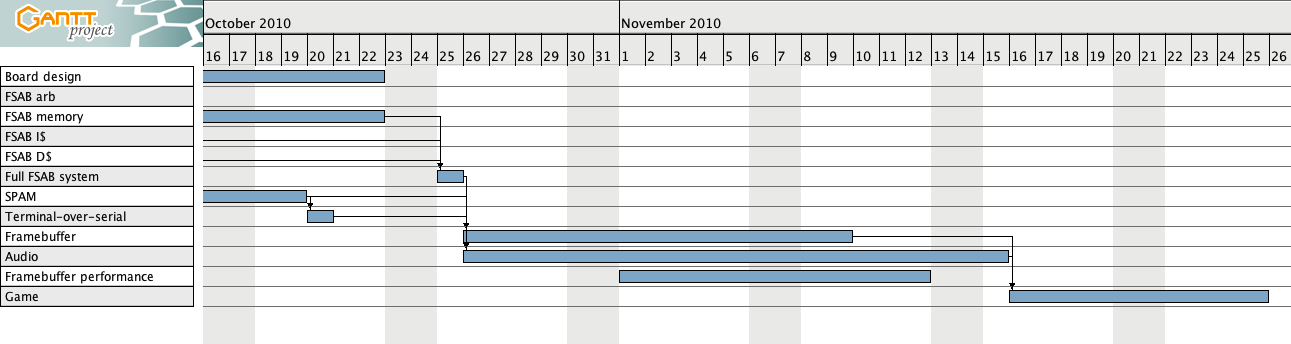
\includegraphics[width=\textwidth]{gantt-chart.png}
  \caption{Mid-semester estimation of schedule.} \label{fig:gantt}
\end{figure}

\section{Individual Team Member Notes}

Pursuant to the requirements of this report, each team member has written a
section on their notes from the class.

\subsection{Joshua Wise}
\label{sec:joshua}

I came into this class at the beginning with one specific goal in mind --
come Hell or high water, I came here to really figure out what it would take
to build a System on a Chip on an FPGA.  Since I learned of the concept of
programmable logic, I dreamed of building a system that was all my own --
every line of code running on it was hand-crafted with care by me (and a few
friends).  So, when I registered for the class, I made this my goal; I would
do what it would take, but this seemed like a prime opportunity to learn as
I would, and learn as I went.

In this regard, I feel as though the course was a success.  On December 3rd,
2010, I walked into HH 1112 with my group members, and got a chance to show
off this system that we had built from the ground up.  All of the C source
on the system was ours; all the assembly was ours; all the RTL was ours; and
to an extent, we even got an opportunity to modify the direct primitives on
the device in debug sessions with FPGA Editor.  There is still plenty more
to do on this project; next semester, the system will be extended to allow
for student 18-447 MIPS cores to be dropped in, and over time, I intend to
build an MMU that will allow me to boot Linux.  Given the time frame that we
had, and the constraints that we faced -- maybe even without taking those
into regard! -- I feel suffused with pride in this accomplishment.

To date, this is the largest project that I have designed from the ground up
on an FPGA.  Our code base spans over 10,000 lines of Verilog (\textit{not}
including the MIG), and nearly 5,000 lines of C; we designed all the
automation for the project, and when we needed something, \textit{we built
it}.  Throughout the course of this, I feel as though all of us have learned
and relearned the value of adhering to a code development methodology; by
sticking to best practices of testing and architecture, we built a
remarkable amount of code that worked right on nearly the first try.

We also rediscovered the relative difficulty of designing RTL with respect
to designing software.  All three of us are accustomed to being able to
write software, designing on the fly, producing a good-quality program in no
time at all; but designing hardware is much more difficult.  I feel as
though we all learned to put our egos aside in development; there may be
less pride in asking for help, but to be sure, there is no pride at all in
code that does not work!  Ultimately, I found over and over again that the
only way to design hardware is to spend a lot of time thinking before I even
touch a keyboard; when doing the first pass of the arbiter, I spent about a
week thinking before I wrote RTL.

What of the class, though?  I felt as though I poured an immense amount of
time and effort into the class, and that that effort went mostly
unappreciated by course staff.  This is a strange feeling for me, as I
usually do not find myself seeking affirmation from the staff of classes I
take.  But in this class, I felt as though I was being actively dismissed by
the course staff; early on in the project, I wrote status reports with
questions, looking for feedback on the direction we were headed.  During the
presentations, I left opportunities open there, too, for feedback and
commentary on our design.  It seems that the feedback never came; it felt as
if the course staff simply did not care to comment on our project. 
Ultimately, the low point of this came when course staff attended our demo
session for what felt like a sum total of 20 minutes; although most of the
members of the class had been in the lab for the previous 48 hours, it
seemed as if course staff was just not interested in the results that we had
produced.

Without regard to the attitudes of the course staff, I still take pride in
the work that I've produced.  I feel as though it took somewhat longer than
it should have to establish a working group dynamic, but once we did so, we
worked as effectively together as any team I have worked with before; when
things needed to happen, they did.  The fact that the three of us were
approximately on par with each other in terms of familiarity with
project-critical features such as version control, scripting, and good
coding practices made our time together that much more enjoyable.

That brings me to a note on which I may wish to end -- advice for future
groups.  Ultimately, what made our group successful is that we embraced our
working environment, instead of holding it at arm's length.  In order to be
successful, we knew that we would have to adopt best practices, and so we
chose a style guide from the first day; we picked a version control system
on day 1, and we set up our computers with an environment that we were
familiar with on day 1.  In order to succeed in this class, you must be
prepared to take advantage of the full power of the tools in front of you;
the RTL is only a place to start.

\textbf{Go forth and build.}

\hfill\textit{Joshua Wise, December 8th, 2010}

\subsection{Josiah Boning}
\label{sec:josiah}

\subsubsection{Things I Liked}

I thoroughly enjoyed our project. I especially liked  the ability to choose 
a project and execute it, the freedom to set up our development environment 
as we like, and the availability of good hardware (development machines and 
FPGA board). I think I learned a lot about designing a large hardware system,
writing RTL (both functionality and style), using \texttt{git}, and how much 
Xilinx sucks. 
One thing to note is that much of the learning I did was either on my own, 
by reading and writing code and solving problems, or from Joshua (section 
\ref{sec:joshua}), who has significant experience doing RTL development and 
is familiar with many quirks of the Xilinx toolchain and other miscellanea. 
His knowldedge of Xilinx, \texttt{git} tricks, and verilog-mode verilator, 
and verilog-mode were invaluable to the project, and I consider the things I 
have learned from his experience to be some of the more significant lessons 
I am taking from this class---so much so that I feel bad for the other groups 
who lack such a verteran RTL developer, as even the TAs did not seem to have 
the same ability to answer obscure questions about Xilinx.\footnote{``It can't 
connect to the USB thing to download the bitfile'' ``Oh, run [obscure xilinx 
command]'' ``...oh.''}

\subsubsection{Things I Didn't Like}

One of the least pleasant things about this class has been the total lack of 
feedback on submitted items. Progress reports, reading summaries, mid-project 
writeup: did anyone read them? Does anyone care? It was impossible to tell. I 
ceased submitting progress reports a month and a half into the semester because 
it truly felt like they were being sent to the void---and I'd rather be working 
on the project than sending things to the void).

\subsubsection{Things I Did}

I worked on our project.

\subsection{Bradley Yoo}

\subsubsection{Joining this team}

I joined this team more than halfway into the class because my previous group wasn't making much progress and one of the members in both groups dropped. When I first joined the group, I was amazed not only by how much RTL has already been written but also by how much more RTL has to be written for the hardware design component of the project to be complete. There were also the software component that we haven't even touched yet.

I was able to be far more productive in the new group than my previous group. I managed to produce more RTL in the first two weeks of joining this project than the previous 2 months I was in the other project. This was mostly because all the other group members worked just as much if not more and the tools were nicely setup. Verilator saved us a couple of times from hours of debugging and verilog-mode was mostly helpful in automating parts of our design process.

\subsubsection{What we did well}

Our group didn't have a set schedule and we were more productive because of it. Every week, we knew we had to get something done so we would decide what is the next highest priority thing to get done, finish it, and then move on. This way, whenever we had a new idea (and we always did), we didn't have to revamp the Gantt chart to consider all the other things that needed to be done. Instead, we implemented it. Modules such as the SimpleDMAReadController and hardware accelerations may not have happened if we didn't have an extremely flexible schedule.

\subsubsection{About the Class}

One of the things that is annoying about this class is the inability of the course staff to give us any help with Xilinx. The TAs were there but they certainly weren't giving us any help with Xilinx in any of the labs. In fact, we rarely met for work in mandatory lab session and instead opted to work overnight because we just got so much more productive because of less noise and more work hours. The lab assignments we had was also useless. The first lab could be done by anyone in 5 minutes because it was just get anything on the board but only one group (this group) managed to get sound on the board because of the lack of documentation and guide inside the lab handout. A 3~4 step procedure on what needs to get done to do the lab just doesn't cut it.

\subsubsection{Conclusion}

I'm very excited that we have managed to produce something that not only works but will be reused for 18-447 (Computer Architecture) next semester. I think that class will become far more meaningful and interesting if the code they produced in class actually ran on the fpga board with display, sound, and keyboard instead of just running on simulation.

\section{In the End}

\begin{verbatim}
joshua@fuggle:~/virtexsquared$ find rtl/ -iname '*.v' -o -iname '*.vh' | \
grep -v mig/ | grep -v chipscope | xargs wc -l | sort -n
     9 rtl/fsab/clog2.vh
    13 rtl/fsab/dma_config_defines.vh
    14 rtl/spam/spam_defines.vh
    32 rtl/fsab/fsab_defines.vh
    38 rtl/core/RegFile.v
    46 rtl/spam/SPAM_Timer.v
    48 rtl/console/SyncGen.v
    63 rtl/util/Fifo.v
    64 rtl/core/Writeback.v
    70 rtl/core/Fetch.v
    73 rtl/fpga/RS232TX.v
    79 rtl/core/ARM_Constants.v
    83 rtl/spam/SPAM_ConsoleIO.v
    91 rtl/util/AsyncFifo.v
    96 rtl/fsab/memory_defines.vh
   100 rtl/fsab/FSABPreload.v
   107 rtl/util/CSRAsyncWrite.v
   108 rtl/util/CSRAsyncRead.v
   114 rtl/audio/ACLink.v
   129 rtl/audio/AC97Conf.v
   131 rtl/fsab/sim/SimpleDMAReadControllerTester.v
   159 rtl/fsab/FSABArbiter.v
   178 rtl/ps2/PS2.v
   217 rtl/spam/SPAM_LCD.v
   221 rtl/console/iic_init.v
   242 rtl/accel/AccelClear.v
   257 rtl/fsab/sim/FSABSimMemory.v
   260 rtl/spam/SPAM_SysACE.v
   304 rtl/fsab/FSABArbiterFIFO.v
   308 rtl/sim/FifoTb.v
   309 rtl/core/Issue.v
   322 rtl/console/Framebuffer.v
   351 rtl/core/Decode.v
   353 rtl/core/ICache.v
   370 rtl/core/DCache.v
   395 rtl/sim/system.v
   398 rtl/accel/AccelBlit.v
   427 rtl/audio/Audio.v
   458 rtl/core/Execute.v
   462 rtl/fsab/SimpleDMAReadController.v
   502 rtl/core/Core.v
   550 rtl/fsab/FSABMemory.v
   796 rtl/fpga/system.v
   861 rtl/core/Memory.v
 10208 total
joshua@fuggle:~/virtexsquared$ find sw -iname '*.[chS]' | grep -v util | \
grep -v res | xargs wc -l  | sort -n
     4 sw/graphics/crt0.S
     6 sw/lib/elfload.h
     7 sw/lib/malloc.h
    11 sw/lib/serial.h
    14 sw/lib/console.h
    16 sw/audio/crt0.S
    16 sw/boot1/crt0.S
    16 sw/fill_perf/crt0.S
    16 sw/game/crt0.S
    16 sw/keyboard/crt0.S
    17 sw/lib/multibuf.h
    18 sw/boot0/crt0.S
    19 sw/lib/qalloc.h
    22 sw/lib/accel.h
    26 sw/lib/stdint.h
    32 sw/lib/doprnt.h
    32 sw/lib/malloc.c
    32 sw/lib/sysace.h
    37 sw/game/gencol.c
    41 sw/lib/audio.h
    42 sw/lib/minilib.h
    49 sw/lib/accel.c
    52 sw/lib/keyhelp.h
    52 sw/lib/multibuf.c
    52 sw/lib/serial.c
    70 sw/keyboard/boot1.c
    73 sw/lib/fat16.h
    76 sw/lib/elfload.c
    78 sw/lib/qalloc.c
    87 sw/boot1/boot1.c
    99 sw/lib/console.c
   101 sw/lib/audio.c
   101 sw/lib/sysace.c
   108 sw/audio/boot1.c
   147 sw/fill_perf/boot1.c
   161 sw/lib/sprintf.c
   202 sw/boot0/charset.h
   203 sw/lib/minilib.c
   221 sw/lib/fat16.c
   239 sw/lib/keyhelp.c
   264 sw/boot0/boot0.c
   288 sw/lib/elf.h
   514 sw/lib/doprnt.c
   786 sw/game/game.c
   813 sw/graphics/boot1.c
  5276 total
\end{verbatim}

\vspace{2.2in}

\center{\Large{Through the fire and the flames, we carry on.}}
\vspace{0.8in}
\center{\textit{Josiah Boning, Joshua Wise, Bradley Yoo}}
\vspace{0.1in}
\center{\textit{December 8, 2010}}

\end{document}
